\documentclass[12pt]{article}
\usepackage{fontspec}
\usepackage{fullpage}
\usepackage{hyperref}
\hypersetup{bookmarks=true,colorlinks=true,linkcolor=red,citecolor=blue,filecolor=magenta,urlcolor=cyan}
\usepackage{amsmath}
\usepackage{amssymb}
\usepackage{mathtools}
\usepackage{unicode-math}
\usepackage{tabularray}
\usepackage{tabularx}
\usepackage{booktabs}
\usepackage{caption}
\usepackage{graphics}
\usepackage{svg}
\usepackage{enumitem}
\usepackage{filecontents}
\usepackage[backend=bibtex]{biblatex}
\usepackage{url}

\usepackage{color}

\newif\ifcomments\commentstrue

\ifcomments
\newcommand{\authornote}[3]{\textcolor{#1}{[#3 ---#2]}}
\newcommand{\todo}[1]{\textcolor{red}{[TODO: #1]}}
\else
\newcommand{\authornote}[3]{}
\newcommand{\todo}[1]{}
\fi

\newcommand{\wss}[1]{\authornote{blue}{SS}{#1}} 

\setmathfont{Latin Modern Math}
\newcommand{\gt}{\ensuremath >}
\newcommand{\lt}{\ensuremath <}
\newlist{symbDescription}{description}{1}
\setlist[symbDescription]{noitemsep, topsep=0pt, parsep=0pt, partopsep=0pt}
\bibliography{bibfile}
\title{Software Requirements Specification for Projectile}
\author{Samuel J. Crawford, Brooks MacLachlan, and W. Spencer Smith}
\begin{document}
\maketitle
\tableofcontents
\newpage
\section{Reference Material}
\label{Sec:RefMat}
This section records information for easy reference.

\subsection{Table of Units}
\label{Sec:ToU}
The unit system used throughout is SI (Système International d'Unités). In addition to the basic units, several derived units are also used. For each unit, the \hyperref[Table:ToU]{Table of Units} lists the symbol, a description, and the SI name.

\begin{longtblr}
[caption={Table of Units}]
{colspec={l l l}, rowhead=1, hline{1,Z}=\heavyrulewidth, hline{2}=\lightrulewidth}
\textbf{Symbol} & \textbf{Description} & \textbf{SI Name}
\\
${\text{m}}$ & length & metre
\\
${\text{rad}}$ & angle & radian
\\
${\text{s}}$ & time & second
\label{Table:ToU}
\end{longtblr}
\subsection{Table of Symbols}
\label{Sec:ToS}
The symbols used in this document are summarized in the
\hyperref[Table:ToS]{Table of Symbols} along with their units. Throughout the
document, symbols in bold will represent vectors, and scalars otherwise. The
symbols are listed in alphabetical order. For vector quantities, the units shown
are for each component of the vector.  \wss{To avoid confusion and to allow for
reuse of symbols with slightly different types (like 3D and 2D vectors), a
separate table of symbols can be generated for each set of theories: background
theories, helper theories, generic theories, projectile theories and final
theories.}

\begin{longtblr}
[caption={Table of Symbols}]
{colspec={l X[l] l}, rowhead=1, hline{1,Z}=\heavyrulewidth, hline{2}=\lightrulewidth}
\textbf{Symbol} & \textbf{Description} & \textbf{Units}
\\
$a$ & Scalar acceleration & $\frac{\text{m}}{\text{s}^{2}}$
\\
${a^{c}}$ & Constant acceleration & $\frac{\text{m}}{\text{s}^{2}}$
\\
${a_{\text{x}}}$ & $x$-component of acceleration & $\frac{\text{m}}{\text{s}^{2}}$
\\
${{a_{\text{x}}}^{\text{c}}}$ & $x$-component of constant acceleration & $\frac{\text{m}}{\text{s}^{2}}$
\\
${a_{\text{y}}}$ & $y$-component of acceleration & $\frac{\text{m}}{\text{s}^{2}}$
\\
${{a_{\text{y}}}^{\text{c}}}$ & $y$-component of constant acceleration & $\frac{\text{m}}{\text{s}^{2}}$
\\
$\symbf{a}\text{(}t\text{)}$ & Acceleration & $\frac{\text{m}}{\text{s}^{2}}$
\\
${\symbf{a}^{\text{c}}}$ & Constant acceleration vector & $\frac{\text{m}}{\text{s}^{2}}$
\\
${d_{\text{offset}}}$ & Distance between the target position and the landing position & ${\text{m}}$
\\
$g$ & Magnitude of gravitational acceleration & $\frac{\text{m}}{\text{s}^{2}}$
\\
$p$ & Scalar position & ${\text{m}}$
\\
$p\text{(}t\text{)}$ & 1D position & ${\text{m}}$
\\
${p^{\text{i}}}$ & Initial position & ${\text{m}}$
\\
${p_{\text{land}}}$ & Landing position & ${\text{m}}$
\\
${p_{\text{target}}}$ & Target position & ${\text{m}}$
\\
${p_{\text{x}}}$ & $x$-component of position & ${\text{m}}$
\\
${{p_{\text{x}}}^{\text{i}}}$ & $x$-component of initial position & ${\text{m}}$
\\
${p_{\text{y}}}$ & $y$-component of position & ${\text{m}}$
\\
${{p_{\text{y}}}^{\text{i}}}$ & $y$-component of initial position & ${\text{m}}$
\\
$\symbf{p}\text{(}t\text{)}$ & Position & ${\text{m}}$
\\
$s$ & Output message as a string & --
\\
$t$ & Time & ${\text{s}}$
\\
${t_{\text{flight}}}$ & Flight duration & ${\text{s}}$
\\
$v$ & Speed & $\frac{\text{m}}{\text{s}}$
\\
$v\text{(}t\text{)}$ & 1D speed & $\frac{\text{m}}{\text{s}}$
\\
${v^{\text{i}}}$ & Initial speed & $\frac{\text{m}}{\text{s}}$
\\
${v_{\text{launch}}}$ & Launch speed & $\frac{\text{m}}{\text{s}}$
\\
${v_{\text{x}}}$ & $x$-component of velocity & $\frac{\text{m}}{\text{s}}$
\\
${{v_{\text{x}}}^{\text{i}}}$ & $x$-component of initial velocity & $\frac{\text{m}}{\text{s}}$
\\
${v_{\text{y}}}$ & $y$-component of velocity & $\frac{\text{m}}{\text{s}}$
\\
${{v_{\text{y}}}^{\text{i}}}$ & $y$-component of initial velocity & $\frac{\text{m}}{\text{s}}$
\\
$\symbf{v}\text{(}t\text{)}$ & Velocity & $\frac{\text{m}}{\text{s}}$
\\
${\symbf{v}^{\text{i}}}$ & Initial velocity & $\frac{\text{m}}{\text{s}}$
\\
$ε$ & Hit tolerance & --
\\
$θ$ & Launch angle & ${\text{rad}}$
\\
$π$ & Ratio of circumference to diameter for any circle & --
\label{Table:ToS}
\end{longtblr}
\subsection{Abbreviations and Acronyms}
\label{Sec:TAbbAcc}
\begin{longtblr}
[caption={Abbreviations and Acronyms}]
{colspec={l l}, rowhead=1, hline{1,Z}=\heavyrulewidth, hline{2}=\lightrulewidth}
\textbf{Abbreviation} & \textbf{Full Form}
\\
1D & One-Dimensional
\\
2D & Two-Dimensional
\\
A & Assumption
\\
DD & Data Definition
\\
GD & General Definition 
\\
GS & Goal Statement
\\
IM & Instance Model
\\
PS & Physical System Description
\\
R & Requirement
\\
RefBy & Referenced by
\\
Refname & Reference Name
\\
SRS & Software Requirements Specification
\\
TM & Theoretical Model
\\
Uncert. & Typical Uncertainty
\label{Table:TAbbAcc}
\end{longtblr}
\section{Introduction}
\label{Sec:Intro}
Projectile motion is a common problem in physics. Therefore, it is useful to have a program to solve and model these types of problems. Common examples of projectile motion include ballistics problems (missiles, bullets, etc.) and the flight of balls in various sports (baseball, golf, football, etc.). The program documented here is called Projectile.

The following section provides an overview of the Software Requirements Specification (SRS) for Projectile. This section explains the purpose of this document, the scope of the requirements, the characteristics of the intended reader, and the organization of the document.

\subsection{Purpose of Document}
\label{Sec:DocPurpose}
The primary purpose of this document is to record the requirements of Projectile. Goals, assumptions, theoretical models, definitions, and other model derivation information are specified, allowing the reader to fully understand and verify the purpose and scientific basis of Projectile. With the exception of \hyperref[Sec:SysConstraints]{system constraints}, this SRS will remain abstract, describing what problem is being solved, but not how to solve it.

This document will be used as a starting point for subsequent development phases, including writing the design specification and the software verification and validation plan. The design document will show how the requirements are to be realized, including decisions on the numerical algorithms and programming environment. The verification and validation plan will show the steps that will be used to increase confidence in the software documentation and the implementation. Although the SRS fits in a series of documents that follow the so-called waterfall model, the actual development process is not constrained in any way. Even when the waterfall model is not followed, as Parnas and Clements point out \cite{parnasClements1986}, the most logical way to present the documentation is still to ``fake'' a rational design process.

\subsection{Scope of Requirements}
\label{Sec:ReqsScope}
The scope of the requirements includes the analysis of a two-dimensional (2D) projectile motion problem with constant acceleration.

\wss{We are only interested in the position of the projectile, not its
orientation \hyperref[SD:noOrient]{SD:noOrient}.} %this is how we leave theories
out, like theories of rotation

\wss{We assume that forces are not relevant for the model so that we only need
kinematic equations \hyperref[SD:kinOnly]{SD:kinOnly}.}

\wss{Relative to ballistics calculations, the scope of Projectile covers
relatively short distances and small magnitude initial velocities
\hyperref[SD:shrtDstSmlMag].} 

\subsection{Characteristics of Intended Reader}
\label{Sec:ReaderChars}
Reviewers of this documentation should have an understanding of undergraduate level 1 physics and undergraduate level 1 calculus. The users of Projectile can have a lower level of expertise, as explained in \hyperref[Sec:UserChars]{Sec:User Characteristics}.

\subsection{Organization of Document}
\label{Sec:DocOrg}
The organization of this document follows the template for an SRS for scientific computing software proposed by \cite{koothoor2013}, \cite{smithLai2005}, \cite{smithEtAl2007}, and \cite{smithKoothoor2016}. The presentation follows the standard pattern of presenting goals, theories, definitions, and assumptions. For readers that would like a more bottom up approach, they can start reading the \hyperref[Sec:IMs]{instance models} and trace back to find any additional information they require.

The \hyperref[Sec:GoalStmt]{goal statements} are refined to the theoretical models and the \hyperref[Sec:TMs]{theoretical models} to the \hyperref[Sec:IMs]{instance models}.

\section{General System Description}
\label{Sec:GenSysDesc}
This section provides general information about the system. It identifies the interfaces between the system and its environment, describes the user characteristics, and lists the system constraints.

\subsection{System Context}
\label{Sec:SysContext}
\hyperref[Figure:sysCtxDiag]{Fig:sysCtxDiag} shows the system context. A circle represents an entity external to the software, the user in this case. A rectangle represents the software system itself (Projectile). Arrows are used to show the data flow between the system and its environment.

\begin{figure}
\begin{center}
\includegraphics[width=\textwidth]{SystemContextFigure.png}
\caption{System Context}
\label{Figure:sysCtxDiag}
\end{center}
\end{figure}
The interaction between the product and the user is through an application programming interface. The responsibilities of the user and the system are as follows:

\begin{itemize}
\item{User Responsibilities}
\begin{itemize}
\item{Provide initial conditions of the physical state of the motion and the input data related to the Projectile, ensuring no errors in the data entry.}
\item{Ensure that consistent units are used for input variables.}
\item{Ensure required \hyperref[Sec:Assumps]{software assumptions} are appropriate for any particular problem input to the software.}
\end{itemize}
\item{Projectile Responsibilities}
\begin{itemize}
\item{Detect data type mismatch, such as a string of characters input instead of a floating point number.}
\item{Determine if the inputs satisfy the required physical and software constraints.}
\item{Calculate the required outputs.}
\end{itemize}
\end{itemize}

\wss{Projectile will be used to explore different scenarios for educational and
learning purposes. It will not be used to perform engineering calculations,
mission-critical or safety-critical applications.} \wss{This additional context
information is needed to determine how much effort should be devoted to the
rationale section.  If the application is safety-critical, the bar is higher.
This is currently less structured, but analogous to, the idea to the Automotive
Safety Integrity Levels (ASILs) that McSCert uses in their automotive hazard
analyses.}

\subsection{User Characteristics}
\label{Sec:UserChars}
The end user of Projectile should have an understanding of high school physics and high school calculus.

\subsection{System Constraints}
\label{Sec:SysConstraints}
There are no system constraints.

\section{Specific System Description}
\label{Sec:SpecSystDesc}
This section first presents the problem description, which gives a high-level view of the problem to be solved. This is followed by the solution characteristics specification, which presents the assumptions, theories, and definitions that are used.

\subsection{Problem Description}
\label{Sec:ProbDesc}
A system is needed to predict whether a launched projectile hits its target.

\subsubsection{Terminology and Definitions}
\label{Sec:TermDefs}
This subsection provides a list of terms that are used in the subsequent sections and their meaning, with the purpose of reducing ambiguity and making it easier to correctly understand the requirements.

\begin{itemize}
\item{Launcher: Where the projectile is launched from and the device that does the launching.}
\item{Projectile: The object to be launched at the target.}
\item{Target: Where the projectile should be launched to.}
\item{Gravity: The force that attracts one physical body with mass to another.}
\item{Cartesian coordinate system: A coordinate system that specifies each point uniquely in a plane by a set of numerical coordinates, which are the signed distances to the point from two fixed perpendicular oriented lines, measured in the same unit of length (from \cite{cartesianWiki}).}
\item{Rectilinear: Occurring \wss{fixed typo in ``Ocurring''} in one dimension.}
\end{itemize}
\subsubsection{Physical System Description}
\label{Sec:PhysSyst}
The physical system of Projectile, as shown in \hyperref[Figure:Launch]{Fig:Launch}, includes the following elements:

\begin{itemize}
\item[PS1:]{The launcher.}
\item[PS2:]{The projectile (with initial velocity ${\symbf{v}^{\text{i}}}$ and launch angle $θ$).}
\item[PS3:]{The target.}
\end{itemize}
\begin{figure}
\begin{center}
\includegraphics[width=0.7\textwidth]{Launch.jpg}
\caption{The physical system}
\label{Figure:Launch}
\end{center}
\end{figure}
\subsubsection{Goal Statements}
\label{Sec:GoalStmt}
Given the initial velocity vector of the projectile and the geometric layout of the launcher and target, the goal statement is:

\begin{itemize} \item[targetHit:\phantomsection\label{targetHit}]{Determine if
the projectile hits the target.} \end{itemize} \subsection{Solution
Characteristics Specification} \label{Sec:SolCharSpec} The instance models that
govern Projectile are presented in the \hyperref[Sec:IMs]{Instance Model
Section}. The information to understand the meaning of the instance models and
their derivation is also presented, so that the instance models can be verified.

\subsubsection{\wss{Types}}

\wss{$\text{time} = \mathbb{R}$} 

\subsubsection{\wss{Scope Decisions}}
\label{Sec:ScopeDec} 

\begin{itemize}
\item[SD:noOrient:\phantomsection\label{SD:noOrient}]{\wss{The orientation of the projectile is ignored. We only care about its translation not its rotation.  (RefBy: \hyperref[Sec:ReqsScope]{Scope of Requirements}).}}
\item[SD:kinOnly:\phantomsection\label{SD:kinOnly}]{\wss{The motion of the
projectile is modelled with only kinematic equations. Forces are not
considered. (RefBy: \hyperref[Sec:ReqsScope]{Scope of Requirements}).}} 
\end{itemize}

\subsubsection{\wss{Modelling Decisions}}
\label{Sec:ModelDec}

\wss{The modelling decisions should likely eventually use a prefix like MD, but
for now most of them will use the prefix A, since that is what was previously
used.}

\begin{itemize}
\item[MD:cartSyst:\phantomsection\label{MD:cartSyst}]{A Cartesian coordinate system is used. (RefBy: \hyperref[TM:acceleration]{TM:acceleration}, \hyperref[TM:velocity]{TM:velocity}, \hyperref[TM:directionCosines]{TM:directionCosines}, \hyperref[GD:rectVel]{GD:rectVel}, \hyperref[GD:rectPos]{GD:rectPos}, \hyperref[GD:velVec]{GD:velVec}, \hyperref[GD:posVec]{GD:posVec}, \hyperref[GD:magAngleToCompRep]{GD:magAngleToCompRep}, \hyperref[PT:coordSyst]{PT:coordSyst}, \hyperref[DD:speedIX]{DD:speedIX}, \hyperref[DD:speedIY]{DD:speedIY}, \hyperref[PT:velVecInitMagAndAngle]{PT:velVecInitMagAndAngle}, \hyperref[PT:posVecInitMagAndAngle]{PT:posVecInitMagAndAngle}, \hyperref[PT:posVecInitPos]{PT:posVecInitPos}, \hyperref[PT:velVecPlanetaryGrav]{PT:velVecPlanetaryGrav}, \hyperref[PT:posVecPlanetaryGrav]{PT:posVecPlanetaryGrav}, \hyperref[IM:calOfLandingTime]{IM:calOfLandingTime}, \hyperref[IM:calOfLandingDist]{IM:calOfLandingDist}, \hyperref[IM:offsetIM]{IM:offsetIM}, and \hyperref[IM:messageIM]{IM:messageIM}.)}
\item[yAxisGravity:\phantomsection\label{yAxisGravity}]{The direction of the $y$-axis is directed opposite to gravity. (RefBy: \hyperref[IM:calOfLandingDist]{IM:calOfLandingDist}, \hyperref[IM:calOfLandingTime]{IM:calOfLandingTime}, \hyperref[IM:messageIM]{IM:messageIM}, \hyperref[PT:posVecInitPos]{PT:posVecInitPos}, \hyperref[IM:offsetIM]{IM:offsetIM}, \hyperref[PT:posVecPlanetaryGrav]{PT:posVecPlanetaryGrav}, \hyperref[PT:velVecPlanetaryGrav]{PT:velVecPlanetaryGrav}, \hyperref[PT:coordSyst]{PT:coordSyst}, \hyperref[PT:posVecInitMagAndAngle]{PT:posVecInitMagAndAngle}, and \hyperref[PT:velVecInitMagAndAngle]{PT:velVecInitMagAndAngle}.)}
\item[launchOrigin:\phantomsection\label{launchOrigin}]{The launcher is coincident with the origin. (RefBy: \hyperref[IM:calOfLandingDist]{IM:calOfLandingDist} and \hyperref[IM:calOfLandingTime]{IM:calOfLandingTime}.)}
\item[targetXAxis:\phantomsection\label{targetXAxis}]{The target lies on the $x$-axis (from \hyperref[neglectCurv]{A:neglectCurv}). (RefBy: \hyperref[IM:calOfLandingTime]{IM:calOfLandingTime}.)}
\item[posXDirection:\phantomsection\label{posXDirection}]{The positive $x$-direction is from the launcher to the target. (RefBy: \hyperref[IM:offsetIM]{IM:offsetIM}, \hyperref[IM:messageIM]{IM:messageIM}, \hyperref[IM:calOfLandingDist]{IM:calOfLandingDist}, and \hyperref[IM:calOfLandingTime]{IM:calOfLandingTime}.)}
\item[timeStartZero:\phantomsection\label{timeStartZero}]{Time starts at zero. (RefBy: \hyperref[GD:velVec]{GD:velVec}, \hyperref[GD:rectVel]{GD:rectVel}, \hyperref[GD:rectPos]{GD:rectPos}, \hyperref[GD:posVec]{GD:posVec}, and \hyperref[IM:calOfLandingTime]{IM:calOfLandingTime}.)}
\item[MD:towardLauncher:\phantomsection\label{MD:towardLauncher}]\wss{The launch velocity is positive. (RefBy: \hyperref[PT:velVecInitMagAndAngle]{PT:velVecInitMagAndAngle})}
\item[MD:magAngleRep:\phantomsection\label{MD:magAngleRep}]\wss{Use the magnitude and angle representation for the initial velocity vector. (RefBy: \hyperref[PT:velVecInitMagAndAngle]{PT:velVecInitMagAndAngle})}

\end{itemize}

\subsubsection{\wss{Background Theory Assumptions}}

\begin{itemize}
\item[threeD:\phantomsection\label{threeD}]{\wss{The motion of the body is in
all three dimensions.} (RefBy: \hyperref[TM:acceleration] {TM:acceleration},
\hyperref[TM:velocity] {TM:velocity}, \hyperref[TM:directionCosines]
{TM:directionCosines})}
\end{itemize}

\subsubsection{\wss{Helper Theory Assumptions (GD:rectVel, GD:rectPos)}}

\begin{itemize}
\item[oneD:\phantomsection\label{oneD}]{The motion of the particle is one dimensional. (RefBy: \hyperref[GD:velVec]{GD:velVec} and \hyperref[GD:posVec]{GD:posVec}.)}
\item[constAccel:\phantomsection\label{constAccel}]{The acceleration is constant (from \hyperref[accelXZero]{A:accelXZero}, \hyperref[accelYGravity]{A:accelYGravity}, \hyperref[neglectDrag]{A:neglectDrag}, and \hyperref[noObstruct]{A:noObstruct}). (RefBy: \hyperref[GD:velVec]{GD:velVec} and \hyperref[GD:posVec]{GD:posVec}.)}
\end{itemize}

\subsubsection{\wss{Generic Theory Assumptions (GD:velVec, GD:posVec)}}

\begin{itemize}
\item[twoD:\phantomsection\label{twoD}]{The variables only depend on
two-dimensions (2D). (RefBy: \hyperref[GD:velVec]{GD:velVec} and
\hyperref[GD:posVec]{GD:posVec}.)} \wss{changed twoDMotion to just twoD, so that
it can be used for things that are 2D other than just the motion.}
\item[constAccelX:\phantomsection\label{constAccelX}]{\wss{The acceleration is constant in the $x$ direction. (RefBy: \hyperref[GD:velVec]{GD:velVec} and \hyperref[GD:posVec]{GD:posVec}.)}}
\item[constAccelY:\phantomsection\label{constAccelY}]{\wss{The acceleration is constant in the $y$ direction. (RefBy: \hyperref[GD:velVec]{GD:velVec} and \hyperref[GD:posVec]{GD:posVec}.)}}
\item[gravAccel:\phantomsection\label{gravAccel}]{\wss{The acceleration is due to gravity. (RefBy: \hyperref[PT:velVecPlanetaryGrav]{PT:velVecPlanetaryGrav} and \hyperref[PT:posVecPlanetaryGrav]{PT:posVecPlanetaryGrav}.)}}

\end{itemize}

\subsubsection{\wss{Projectile Specific Theory Assumptions}}

\begin{itemize}
\item[accelXZero:\phantomsection\label{accelXZero}]{The constant acceleration in
the $x$-direction is zero. (RefBy:
\hyperref[IM:calOfLandingDist]{IM:calOfLandingDist} and
\hyperref[constAccel]{A:constAccel}.)}
\item[accelYGravity:\phantomsection\label{accelYGravity}]{The constant
acceleration in the $y$-direction is the acceleration due to gravity (from
\hyperref[yAxisGravity]{A:yAxisGravity}). (RefBy:
\hyperref[IM:calOfLandingTime]{IM:calOfLandingTime} and
\hyperref[constAccel]{A:constAccel}).}
\item[gravAccelValue:\phantomsection\label{gravAccelValue}]{The acceleration due
to gravity is assumed to have the value provided in the section for
\hyperref[Sec:AuxConstants]{Values of Auxiliary Constants}. (RefBy:
\hyperref[IM:calOfLandingDist]{IM:calOfLandingDist} and
\hyperref[IM:calOfLandingTime]{IM:calOfLandingTime}.)}
\item[noObstruct:\phantomsection\label{noObstruct}]{No obstructions impede the path of the projectile.  This means there is nothing rising from the ground that will block the flight and no other projectiles collide with the launched projectile. (RefBy: \hyperref[PT:coordSyst]{PT:coordSyst}, \hyperref[IM:calOfLandingDist]{IM:calOfLandingDist}, etc.)}
\item[flatPlanet:\phantomsection\label{flatPlanet}]{No surface of the planet is assummed flat; that is, there is assumed to be no curvature. (RefBy: \hyperref[PT:coordSyst]{PT:coordSyst}, \hyperref[IM:calOfLandingDist]{IM:calOfLandingDist}, etc.)}

\end{itemize}

\subsubsection{\wss{Rationale Assumptions}}

\begin{itemize}
\item[centreMass:\phantomsection\label{centreMass}]{We only care about the motion of the centre of mass of the projectile. (RefBy: Section~\ref{Sec:SDRationale})}
\item[neglectCurv:\phantomsection\label{neglectCurv}]{The distance is small enough that the curvature of the celestial body can be neglected. (RefBy: \hyperref[targetXAxis]{A:targetXAxis} and \hyperref[MD:cartSyst]{MD:cartSyst}.)}
\item[neglectDrag:\phantomsection\label{neglectDrag}]{Air drag is neglected. (RefBy: \hyperref[constAccel]{A:constAccel}.)}
\item[negPlanetRot:\phantomsection\label{negEarthRot}]{\wss{The rotation of the
planet is neglected}. (RefBy: ?)}

\end{itemize}

\subsubsection{\wss{Context Theories}}

\wss{In science and engineering the theories that are used to solve practical
problems are built on a foundation of mathematical and physical knowledge. For
practical reasons, it is not usually feasible to define all of the details down
to the most fundamental level. For instance, the audience reading the
requirements will typically know the concepts of real arithmetic,
differentiation, trigonometry, etc.  Nevertheless it is helpful to make the
dependence on fundamental theories explicit, even if those theories themselves
are not explicitly defined. These theories form the context in which the higher
level theories exist.  The context theories that are used for the Projectile
problem are listed below.}

\medskip
\noindent
\begin{minipage}{\textwidth}
\begin{tabular}{>{\raggedright}p{0.13\textwidth}>{\raggedright\arraybackslash}p{0.82\textwidth}}
\toprule \textbf{Refname} & \textbf{\wss{CT:realArith}}
\phantomsection 
\label{CT:realArith}
\\ \midrule
Label & Real Arithmetic
\\ \midrule
Source & \cite{}
\\ \midrule
RefBy & \hyperref[TM:acceleration]{TM:acceleration},
\hyperref[TM:velocity]{TM:velocity},
\hyperref[TM:directionCosines]{TM:directionCosines},
\hyperref[GD:rectVel]{GD:rectVel}, \hyperref[GD:rectVel]{GD:rectVel}, \hyperref[DD:speedIX]{DD:speedIX}, \hyperref[DD:speedIY]{DD:speedIY},everything (TODO: not complete; almost every theory uses this context theory.)
\\ \bottomrule
\end{tabular}
\end{minipage}
~\\

\medskip
\noindent
\begin{minipage}{\textwidth}
\begin{tabular}{>{\raggedright}p{0.13\textwidth}>{\raggedright\arraybackslash}p{0.82\textwidth}}
\toprule \textbf{Refname} & \textbf{\wss{CT:trigonometry}}
\phantomsection 
\label{CT:trigonometry}
\\ \midrule
Label & Trigonometry
\\ \midrule
Source & \cite{}
\\ \midrule
RefBy & \hyperref[TM:directionCosines]{TM:directionCosines}, \hyperref[DD:speedIX]{DD:speedIX}, \hyperref[DD:speedIY]{DD:speedIY},everything (TODO: fill in)
\\ \bottomrule
\end{tabular}
\end{minipage}
~\\

\medskip
\noindent
\begin{minipage}{\textwidth}
\begin{tabular}{>{\raggedright}p{0.13\textwidth}>{\raggedright\arraybackslash}p{0.82\textwidth}}
\toprule \textbf{Refname} & \textbf{\wss{CT:vectors}}
\phantomsection 
\label{CT:vectors}
\\ \midrule
Label & Vectors
\\ \midrule
Source & \cite{}
\\ \midrule
RefBy & \hyperref[TM:acceleration]{TM:acceleration},
\hyperref[TM:velocity]{TM:velocity},
\hyperref[TM:directionCosines]{TM:directionCosines},
\hyperref[GD:rectVel]{GD:rectVel}, \hyperref[GD:rectVel]{GD:rectVel}, \hyperref[DD:speedIX]{DD:speedIX}, \hyperref[DD:speedIY]{DD:speedIY},TODO: fill in
\\ \bottomrule
\end{tabular}
\end{minipage}
~\\

\medskip
\noindent
\begin{minipage}{\textwidth}
\begin{tabular}{>{\raggedright}p{0.13\textwidth}>{\raggedright\arraybackslash}p{0.82\textwidth}}
\toprule \textbf{Refname} & \textbf{\wss{CT:CartCoordSyst}}
\phantomsection 
\label{CT:CartCoordSyst}
\\ \midrule
Label & Cartesian Coordinate System
\\ \midrule
Source & \cite{}
\\ \midrule
RefBy & \hyperref[TM:acceleration]{TM:acceleration},
\hyperref[TM:velocity]{TM:velocity},
\hyperref[TM:directionCosines]{TM:directionCosines},
\hyperref[GD:rectVel]{GD:rectVel}, \hyperref[GD:rectVel]{GD:rectVel}, \hyperref[DD:speedIX]{DD:speedIX}, \hyperref[DD:speedIY]{DD:speedIY},TODO: fill in
\\ \bottomrule
\end{tabular}
\end{minipage}
~\\

\medskip
\noindent
\begin{minipage}{\textwidth}
\begin{tabular}{>{\raggedright}p{0.13\textwidth}>{\raggedright\arraybackslash}p{0.82\textwidth}}
\toprule \textbf{Refname} & \textbf{\wss{CT:Differentiation}}
\phantomsection 
\label{CT:Differentiation}
\\ \midrule
Label & Differentiation
\\ \midrule
Source & \cite{}
\\ \midrule
RefBy & \hyperref[TM:acceleration]{TM:acceleration},
\hyperref[TM:velocity]{TM:velocity}, \hyperref[GD:rectVel]{GD:rectVel}, \hyperref[GD:rectVel]{GD:rectVel}, TODO:
fill in 
\\ \bottomrule
\end{tabular}
\end{minipage}
~\\

\medskip
\noindent
\begin{minipage}{\textwidth}
\begin{tabular}{>{\raggedright}p{0.13\textwidth}>{\raggedright\arraybackslash}p{0.82\textwidth}}
\toprule \textbf{Refname} & \textbf{\wss{CT:Integration}}
\phantomsection 
\label{CT:Integration}
\\ \midrule
Label & Integration
\\ \midrule
Source & \cite{}
\\ \midrule
RefBy & \hyperref[GD:rectVel]{GD:rectVel}, TODO: fill in
\\ \bottomrule
\end{tabular}
\end{minipage}
~\\

\subsubsection{\wss{Background Theories (BT)}}
\label{Sec:TMs}
This section focuses on the general equations and laws that Projectile is based
on.  \wss{Maybe relabel all of the background theories with the prefix BT,
instead of TM?}

\medskip
\noindent
\begin{minipage}{\textwidth}
\begin{tabular}{>{\raggedright}p{0.13\textwidth}>{\raggedright\arraybackslash}p{0.82\textwidth}}
\toprule \textbf{Refname} & \textbf{TM:acceleration}
\phantomsection 
\label{TM:acceleration}
\\ \midrule
Label & Acceleration
\\ \midrule
Equation & \begin{displaymath}
           \symbf{a}\text{(}t\text{)}=\frac{\,d\symbf{v}\text{(}t\text{)}}{\,dt}
           \end{displaymath}
\\ \midrule
Description & \begin{symbDescription}
              \item{\wss{$t: \text{time}$} is the time (${\text{s}}$)}
              \item{\wss{$\symbf{a}: \text{time} \rightarrow \mathbb{R}^3$} is the acceleration ($\frac{\text{m}}{\text{s}^{2}}$)}
              \item{\wss{$\symbf{v}: \text{time} \rightarrow \mathbb{R}^3$} is the velocity ($\frac{\text{m}}{\text{s}}$)}
              \end{symbDescription}
\\ \midrule
\wss{Constraints} & \wss{None}

\\ \midrule
Notes & The velocity and acceleration of the body are expressed using a 3D
(\hyperref[threeD]{A:threeD}) Cartesian coordinate system
(\hyperref[CT:CartCoordSyst]{CT:CartCoordSyst},
\hyperref[MD:cartSyst]{MD:cartSyst}).  That is, the coordinate system is
rectangular (orthonormal). The relationship between acceleration and velocity
uses the concepts of real arithmetic, vectors and differentiation
(\hyperref[CT:realArith]{CT:realArith}, \hyperref[CT:vectors]{CT:vectors},
\hyperref[CT:Differentiation]{CT:Differentiation}).

\\ \midrule
Source & \cite{accelerationWiki}
         
\\ \midrule
RefBy & \hyperref[GD:rectVel]{GD:rectVel}
        
\\ \bottomrule
\end{tabular}
\end{minipage}
~\\
\noindent \textbf{Context Theories Used by TM:acceleration}

\begin{itemize}
\item \hyperref[CT:realArith]{CT:realArith}
\item \hyperref[CT:vectors]{CT:vectors}
\item \hyperref[CT:CartCoordSyst]{CT:CartCoodSyst}
\item \hyperref[CT:Differentiation]{CT:Differentiation}
\end{itemize}

\noindent \textbf{Initial Theories Used by TM:acceleration}

None
~\\

\noindent \textbf{Preconditions for TM:acceleration}

\begin{itemize}
\item \hyperref[MD:cartSyst]{MD:cartSyst}
\item \hyperref[threeD]{A:threeD}
\end{itemize}

\medskip
\noindent
\begin{minipage}{\textwidth}
\begin{tabular}{>{\raggedright}p{0.13\textwidth}>{\raggedright\arraybackslash}p{0.82\textwidth}}
\toprule \textbf{Refname} & \textbf{TM:velocity}
\phantomsection 
\label{TM:velocity}
\\ \midrule
Label & Velocity
        
\\ \midrule
Equation & \begin{displaymath}
           \symbf{v}\text{(}t\text{)}=\frac{\,d\symbf{p}\text{(}t\text{)}}{\,dt}
           \end{displaymath}
\\ \midrule
Description & \begin{symbDescription}
              \item{\wss{$t: \text{time}$} is the time (${\text{s}}$)}
              \item{\wss{$\symbf{v}: \text{time} \rightarrow \mathbb{R}^3$} is the velocity ($\frac{\text{m}}{\text{s}}$)}
              \item{\wss{$\symbf{p}: \text{time} \rightarrow \mathbb{R}^3$} is the position (${\text{m}}$)}
              \end{symbDescription}
\\ \midrule
\wss{Constraints} & \wss{None}

\\ \midrule
Notes & The position and velocity of the body are expressed using a 3D (\hyperref[threeD]{A:threeD}) Cartesian
coordinate system (\hyperref[CT:CartCoordSyst]{CT:CartCoordSyst},
\hyperref[MD:cartSyst]{MD:cartSyst}).  That is, the coordinate system is rectangular
(orthonormal).  The relationship between velocity and position uses the concepts
of real arithmetic, vectors and differentiation
(\hyperref[CT:realArith]{CT:realArith}, \hyperref[CT:vectors]{CT:vectors},
\hyperref[CT:Differentiation]{CT:Differentiation}).

\\ \midrule
Source & \cite{velocityWiki}
         
\\ \midrule
RefBy & \hyperref[GD:rectPos]{GD:rectPos}
        
\\ \bottomrule
\end{tabular}
\end{minipage}
~\\
\noindent \textbf{Context Theories Used by TM:velocity}

\begin{itemize}
\item \hyperref[CT:realArith]{CT:realArith}
\item \hyperref[CT:vectors]{CT:vectors}
\item \hyperref[CT:CartCoordSyst]{CT:CartCoodSyst}
\item \hyperref[CT:Differentiation]{CT:Differentiation}
\end{itemize}

\noindent \textbf{Initial Theories Used by TM:velocity}

None
~\\

\noindent \textbf{Preconditions for TM:velocity}

\begin{itemize}
\item \hyperref[MD:cartSyst]{MD:cartSyst}
\item \hyperref[threeD]{A:threeD}
\end{itemize}

\medskip
\noindent
\begin{minipage}{\textwidth}
\begin{tabular}{>{\raggedright}p{0.13\textwidth}>{\raggedright\arraybackslash}p{0.82\textwidth}}
\toprule \textbf{Refname} & \textbf{TM:directionCosines}
\phantomsection 
\label{TM:directionCosines}
\\ \midrule
Label & \wss{Direction Cosines Representation for Vectors}
\\ \midrule   
Equation & \begin{displaymath}
           b_x = |\symbf{b}| \cos (\alpha), b_y = |\symbf{b}| \cos (\beta), b_z
           = |\symbf{b}| \cos (\gamma)
           \end{displaymath}
\\ \midrule
Description & \begin{symbDescription}
              \item \wss{$\alpha: \mathbb{R}$} is the angle between the vector and the positive $x$ axis 
              \item \wss{$\beta: \mathbb{R}$} is the angle between the vector and the positive $y$ axis 
              \item \wss{$\gamma: \mathbb{R}$} is the angle between the vector and the positive $z$ axis 
              \item \wss{$|\symbf{b}|: \mathbb{R}$} is the magnitude of the vector
              \item \wss{$b_x: \mathbb{R}$} is the $x$ component of the vector $\symbf{b}$
              \item \wss{$b_y: \mathbb{R}$} is the $y$ component of the vector $\symbf{b}$
              \item \wss{$b_z: \mathbb{R}$} is the $z$ component of the vector $\symbf{b}$
              \end{symbDescription}

\\ \midrule
\wss{Constraints} & \wss{$\cos^2(\alpha) + \cos^2(\beta) + \cos^2(\gamma) = 1$}

\\ \midrule
Notes & \wss{The vector $\symbf{b}$ is in a 3D (\hyperref[threeD]{A:threeD})
Cartesian coordinate system (\hyperref[CT:CartCoordSyst]{CT:CartCoordSyst},
\hyperref[MD:cartSyst]{MD:cartSyst}).}  \wss{A figure showing the angles for a
sample vector would be a nice addition.}  Direction cosines use the context
theories of real arithmetic, trigonometry and vectors
(\hyperref[CT:realArith]{CT:realArith},
\hyperref[CT:trigonometry]{CT:trigonometry}, \hyperref[CT:vectors]{CT:vectors}).

\\ \midrule
Source & \cite{} \href{https://byjus.com/maths/direction-cosines/} {web-page
resource}, Long book 
         
\\ \midrule
RefBy & \hyperref[GD:magAngleToCompRep]{GD:magAngleToCompRep}
        
\\ \bottomrule
\end{tabular}
\end{minipage}
~\\
\noindent \textbf{Context Theories Used by TM:directionCosines}

\begin{itemize}
\item \hyperref[CT:realArith]{CT:realArith}
\item \hyperref[CT:trigonometry]{CT:trigonometry}
\item \hyperref[CT:CartCoordSyst]{CT:CartCoordSyst}
\item \hyperref[CT:vectors]{CT:vectors}
\end{itemize}

\noindent \textbf{Initial Theories Used by TM:directionCosines}

None
~\\

\noindent \textbf{Preconditions for TM:directionCosines}

\begin{itemize}
\item \hyperref[MD:cartSyst]{MD:cartSyst}
\item \hyperref[threeD]{A:threeD}
\end{itemize}

\subsubsection{\wss{Helper Theories (GD:rectVel and GD:rectPos)}}
\label{Sec:GDs}
This section collects the laws and equations that will be used to build the instance models.
\wss{We should remove the prefix GD.  Maybe we should replace it with the prefix
TM?}
\medskip
\noindent
\begin{minipage}{\textwidth}
\begin{tabular}{>{\raggedright}p{0.13\textwidth}>{\raggedright\arraybackslash}p{0.82\textwidth}}
\toprule \textbf{Refname} & \textbf{GD:rectVel}
\phantomsection 
\label{GD:rectVel}
\\ \midrule
Label & Rectilinear (1D) velocity as a function of time for constant acceleration
        
\\ \midrule
Units & $\frac{\text{m}}{\text{s}}$ \wss{Do we need units as a separate field? user option?}
\\ \midrule
Equation & \begin{displaymath}
           v\text{(}t\text{)}={v^{\text{i}}}+{a^{c}} t
           \end{displaymath}
\\ \midrule
Description & \begin{symbDescription}
              \item{\wss{$v: \text{time} \rightarrow \mathbb{R}$} is the 1D speed ($\frac{\text{m}}{\text{s}}$)}
              \item{\wss{${v^{\text{i}}: \mathbb{R}}$} is the initial speed ($\frac{\text{m}}{\text{s}}$)}
              \item{\wss{${a^{c}: \mathbb{R}}$} is the constant acceleration ($\frac{\text{m}}{\text{s}^{2}}$)}
              \item{\wss{$t: \text{time}$} is the time (${\text{s}}$)}
              \end{symbDescription}

\\ \midrule
\wss{Constraints} & \wss{$t \geq 0$}
\wss{\hyperref[timeStartZero]{A:timeStartZero}} 

\\ \midrule
\wss{Notes} & \wss{See detailed derivation of equation and constraint below}

\\ \midrule
Source & \cite[(pg. 8)]{hibbeler2004}
         
\\ \midrule
RefBy & \hyperref[GD:velVec]{GD:velVec}% and \hyperref[GD:rectPos]{GD:rectPos}
        
\\ \bottomrule
\end{tabular}
\end{minipage}

\paragraph{Detailed derivation of rectilinear velocity:}
\label{GD:rectVelDeriv}
\wss{We start from the theory of acceleration
\hyperref[TM:acceleration]{TM:acceleration} for a body in 3D Cartesian space:}

$$\symbf{a}\text{(}t\text{)}=\frac{\,d\symbf{v}\text{(}t\text{)}}{\,dt}$$

\wss{At this point we change the assumption of 3D motion
(\hyperref[threeD]{A:threeD}) to instead assume the body only travels in a
straight line along one dimension of the coordinate system
(\hyperref[oneD]{A:oneD}):}

$${a}\text{(}t\text{)}=\frac{\,d{v}\text{(}t\text{)}}{\,dt}$$

\wss{We now assume that the acceleration is constant (does not vary with time)
(\hyperref[constAccel]{A:constAccel}) represented by ${a^{c}}$. The initial
velocity (at $t=0$, from \hyperref[timeStartZero]{A:timeStartZero}) is
represented by ${v^{\text{i}}}$. We now have:}

\begin{displaymath}
{a^{c}}=\frac{\,dv}{\,dt}
\end{displaymath}
Rearranging and integrating, we have:

\begin{displaymath}
\int_{{v^{\text{i}}}}^{v}{1}\,dv=\int_{0}^{t}{{a^{c}}}\,dt
\end{displaymath}
Performing the integration, we have the required equation:

\begin{displaymath}
v\text{(}t\text{)}={v^{\text{i}}}+{a^{c}} t
\end{displaymath}

\wss{The theory for rectilinear velocity uses the context theories from
\hyperref[TM:acceleration]{TM:acceleration} of real arithmetic, vectors,
Cartesian coodinate system, and differentiation
(\hyperref[CT:realArith]{CT:realArith}, \hyperref[CT:vectors]{CT:vectors},
\hyperref[CT:CartCoordSyst]{CT:CartCoordSyst},
\hyperref[CT:Differentiation]{CT:Differentiation}).  In addition, the context
theory of integration is used (\hyperref[CT:Integration]{CT:Integration}).}

\paragraph{Detailed derivation of constraints for GD:rectVel:}

\wss{The data constraint that $t \geq 0$ comes from the assumption that times
starts at zero (\hyperref[timeStartZero]{A:timeStartZero}); that is, the initial
velocity applies at $t=0$.  Therefore, the equation is nonsensical for
negative time.}
~\\

\noindent \textbf{Context Theories Used by GD:rectVel}

\begin{itemize}
\item \hyperref[CT:realArith]{CT:realArith}
\item \hyperref[CT:vectors]{CT:vectors}
\item \hyperref[CT:CartCoordSyst]{CT:CartCoordSyst}
\item \hyperref[CT:Differentiation]{CT:Differentiation}
\item \hyperref[CT:Integration]{CT:Integration}
\end{itemize}

\noindent \textbf{Initial Theories Used by GD:rectVel}

\begin{itemize}
\item \hyperref[TM:acceleration]{TM:acceleration}
\end{itemize}

\noindent \textbf{\wss{Preconditions for GD:rectVel}}

\begin{itemize}
\item \hyperref[MD:cartSyst]{MD:cartSyst} (inherited from \hyperref[TM:acceleration]{TM:acceleration})
\item \hyperref[oneD]{A:oneD} (overrides \hyperref[threeD]{A:threeD})
\item \hyperref[constAccel]{A:constAccel}
\item \hyperref[timeStartZero]{A:timeStartZero}
\end{itemize}

\medskip
\noindent
\begin{minipage}{\textwidth}
\begin{tabular}{>{\raggedright}p{0.13\textwidth}>{\raggedright\arraybackslash}p{0.82\textwidth}}
\toprule \textbf{Refname} & \textbf{GD:rectPos}
\phantomsection 
\label{GD:rectPos}
\\ \midrule
Label & Rectilinear (1D) position as a function of time for constant acceleration
        
\\ \midrule
Units & ${\text{m}}$
        
\\ \midrule
Equation & \begin{displaymath}
           p\text{(}t\text{)}={p^{\text{i}}}+{v^{\text{i}}} t+\frac{{a^{c}} t^{2}}{2}
           \end{displaymath}

\\ \midrule
Description & \begin{symbDescription}
              \item{\wss{$p: \text{time} \rightarrow \mathbb{R}$} is the 1D position (${\text{m}}$)}
              \item{\wss{${p^{\text{i}}}: \mathbb{R}$} is the initial position (${\text{m}}$)}
              \item{\wss{${v^{\text{i}}}: \mathbb{R}$} is the initial speed ($\frac{\text{m}}{\text{s}}$)}
              \item{\wss{$t: \mathbb{R}$} is the time (${\text{s}}$)}
              \item{\wss{${a^{c}}: \mathbb{R}$} is the constant acceleration ($\frac{\text{m}}{\text{s}^{2}}$)}
              \end{symbDescription}
\\ \midrule
\wss{Constraints} & \wss{$t \geq 0$} \wss{\hyperref[timeStartZero]{A:timeStartZero}}

\\ \midrule
\wss{Notes} & \wss{See detailed derivation of equation and constraint below}

\\ \midrule
Source & \cite[(pg. 8)]{hibbeler2004}
         
\\ \midrule
RefBy & \hyperref[GD:posVec]{GD:posVec}
        
\\ \bottomrule
\end{tabular}
\end{minipage}

\paragraph{Detailed derivation of rectilinear position:}
\label{GD:rectPosDeriv}
\wss{We start from the kinematic equation for velocity
\hyperref[TM:velocity]{TM:velocity} for a body in 3D Cartesian space:}

$$\symbf{v}\text{(}t\text{)}=\frac{\,d\symbf{p}\text{(}t\text{)}}{\,dt}$$

\wss{At this point we assume the body only travels in a straight line along one
dimension of the coordinate system (\hyperref[oneD]{A:oneD}):}

$${v}\text{(}t\text{)}=\frac{\,d{p}\text{(}t\text{)}}{\,dt}$$

\wss{The initial position (at $t=0$, from
\hyperref[timeStartZero]{A:timeStartZero}) is represented by ${p^{\text{i}}}$.
Rearranging the above equation and integrating we have:}

\begin{displaymath}
\int_{{p^{\text{i}}}}^{p(t)}{1}\,dp=\int_{0}^{t}{v(t)}\,dt
\end{displaymath}
\wss{This equation has been changed from the previous version to show $p(t)$ and
$v(t)$}

\wss{We now assume that the acceleration is constant (does not vary with time)
(\hyperref[constAccel]{A:constAccel}) represented by ${a^{c}}$. The initial
velocity (at $t=0$, from \hyperref[timeStartZero]{A:timeStartZero}) is
represented by ${v^{\text{i}}}$. Since we satisfy the preconditions for
\hyperref[GD:rectVel]{GD:rectVel} we can replace $v(t)$ to get:}

\begin{displaymath}
\int_{{p^{\text{i}}}}^{p(t)}{1}\,dp=\int_{0}^{t}{{v^{\text{i}}}+{a^{c}} t}\,dt
\end{displaymath}
\wss{The above equation has been changed from the previous version to show
$p(t)$.}
Performing the integration, we have the required equation:

\begin{displaymath}
p\text{(}t\text{)}={p^{\text{i}}}+{v^{\text{i}}} t+\frac{{a^{c}} t^{2}}{2}
\end{displaymath}

\wss{The theory for rectilinear position uses the context theories from
\hyperref[TM:acceleration]{TM:acceleration} of real arithmetic, vectors,
Cartesian coodinate system, and differentiation
(\hyperref[CT:realArith]{CT:realArith}, \hyperref[CT:vectors]{CT:vectors},
\hyperref[CT:CartCoordSyst]{CT:CartCoordSyst},
\hyperref[CT:Differentiation]{CT:Differentiation}).  In addition, the context
theory of integration is used (\hyperref[CT:Integration]{CT:Integration}).}

\paragraph{Detailed derivation of constraints for GD:rectPos:}

\wss{The data constraint that $t \geq 0$ comes from the assumption that times
starts at zero (\hyperref[timeStartZero]{A:timeStartZero}); that is, the initial
velocity applies at $t=0$.  Therefore, the equation is nonsensical for
negative time.}
~\\

\noindent \textbf{Context Theories Used by GD:rectPos}

\begin{itemize}
\item \hyperref[CT:realArith]{CT:realArith}
\item \hyperref[CT:vectors]{CT:vectors}
\item \hyperref[CT:CartCoordSyst]{CT:CartCoordSyst}
\item \hyperref[CT:Differentiation]{CT:Differentiation}
\item \hyperref[CT:Integration]{CT:Integration}
\end{itemize}

\noindent \textbf{Initial Theories Used by GD:rectPos}

\begin{itemize}
\item \hyperref[TM:velocity]{TM:velocity}
\end{itemize}

\noindent \textbf{Preconditions for GD:rectPos}

\begin{itemize}
\item \hyperref[MD:cartSyst]{MD:cartSyst} (inherited from \hyperref[TM:velocity]{TM:velocity})
\item \hyperref[oneD]{A:oneD}
\item \hyperref[constAccel]{A:constAccel}
\item \hyperref[timeStartZero]{A:timeStartZero}
\end{itemize}

\subsubsection{\wss{Generic Theories (GD:velVec and GD:posVec)}}

\noindent
\begin{minipage}{\textwidth}
\begin{tabular}{>{\raggedright}p{0.13\textwidth}>{\raggedright\arraybackslash}p{0.82\textwidth}}
\toprule \textbf{Refname} & \textbf{GD:velVec}
\phantomsection 
\label{GD:velVec}
\\ \midrule
Label & Velocity vector as a function of time for 2D motion under constant acceleration
        
\\ \midrule
Units & $\frac{\text{m}}{\text{s}}$
        
\\ \midrule
Equation & \begin{displaymath}
           \symbf{v}\text{(}t\text{)}=\begin{bmatrix}
                                      {{v_{\text{x}}}^{\text{i}}}+{{a_{\text{x}}}^{\text{c}}} t\\
                                      {{v_{\text{y}}}^{\text{i}}}+{{a_{\text{y}}}^{\text{c}}} t
                                      \end{bmatrix}
           \end{displaymath}
\\ \midrule
Description & \begin{symbDescription}
              \item{\wss{$\symbf{v}: \text{time} \rightarrow \mathbb{R}^2$} is the velocity \wss{vector} ($\frac{\text{m}}{\text{s}}$)}
              \item{\wss{${{v_{\text{x}}}^{\text{i}}}: \mathbb{R}$} is the $x$-component of initial velocity ($\frac{\text{m}}{\text{s}}$)}
              \item{\wss{${{a_{\text{x}}}^{\text{c}}}: \mathbb{R}$} is the $x$-component of constant acceleration ($\frac{\text{m}}{\text{s}^{2}}$)}
              \item{\wss{$t$: \text{time}} is the time (${\text{s}}$)}
              \item{\wss{${{v_{\text{y}}}^{\text{i}}}: \mathbb{R}$} is the $y$-component of initial velocity ($\frac{\text{m}}{\text{s}}$)}
              \item{\wss{${{a_{\text{y}}}^{\text{c}}}: \mathbb{R}$} is the $y$-component of constant acceleration ($\frac{\text{m}}{\text{s}^{2}}$)}
              \end{symbDescription}
\\ \midrule

\wss{Constraints} & \wss{$t \geq 0$} \wss{Inherited from
\hyperref[GD:rectVel]{GD:rectVel}}
\\ \midrule

Source & --
         
\\ \midrule
RefBy & \hyperref[PT:velVecInitMagAndAngle]{PT:velVecInitMagAndAngle}
\\ \bottomrule
\end{tabular}
\end{minipage}

\paragraph{Detailed derivation of velocity vector:}
\label{GD:velVecDeriv}
For a two-dimensional Cartesian coordinate system (\hyperref[twoD]{A:twoD} and \hyperref[MD:cartSyst]{MD:cartSyst}), we can represent the velocity vector as $\symbf{v}\text{(}t\text{)}=\begin{bmatrix}
                                                                                                                                                                                                 {v_{\text{x}}(\wss{t})}\\
                                                                                                                                                                                                 {v_{\text{y}}(\wss{t})}
                                                                                                                                                                                                 \end{bmatrix}$ and the acceleration vector as $\symbf{a}\text{(}t\text{)}=\begin{bmatrix}
                                                                                                                                                                                                                                                                           {a_{\text{x}}(\wss{t})}\\
                                                                                                                                                                                                                                                                           {a_{\text{y}}(\wss{t})}
                                                                                                                                                                                                                                                                           \end{bmatrix}$. The acceleration is assumed to be constant in both the $x$ direction ${a_{\text{x}}}^{\text{c}}$ (\hyperref[constAccelX]{A:constAccelX}) and $y$ direction ${a_{\text{y}}}^{\text{c}}$ (\hyperref[constAccelY]{A:constAccelY}). The constant acceleration vector is represented as ${\symbf{a}^{\text{c}}}=\begin{bmatrix}
                                                                                                                                                                                                                                                                                                                                                                                                                                                           {{a_{\text{x}}}^{\text{c}}}\\
                                                                                                                                                                                                                                                                                                                                                                                                                                                           {{a_{\text{y}}}^{\text{c}}}
                                                                                                                                                                                                                                                                                                                                                                                                                                                           \end{bmatrix}$. The initial velocity (at $t=0$, from \hyperref[timeStartZero]{A:timeStartZero}) is represented by ${\symbf{v}^{\text{i}}}=\begin{bmatrix}
                                                                                                                                                                                                                                                                                                                                                                                                                                                                                                                                                                                                     {{v_{\text{x}}}^{\text{i}}}\\
                                                                                                                                                                                                                                                                                                                                                                                                                                                                                                                                                                                                     {{v_{\text{y}}}^{\text{i}}}
                                                                                                                                                                                                                                                                                                                                                                                                                                                                                                                                                                                                     \end{bmatrix}$. \wss{For each coordinate direction we satisfy the preconditions for \hyperref[GD:rectVel]{GD:rectVel} (\hyperref[MD:cartSyst]{MD:cartSyst}, \hyperref[oneD]{A:oneD}, \hyperref[constAccel]{A:constAccel}, \hyperref[timeStartZero]{A:timeStartZero}). This means we can use the one dimensional equation for each of the two coordinate directions to yield the required equation:}

\begin{displaymath}
\symbf{v}\text{(}t\text{)}=\begin{bmatrix}
                           {{v_{\text{x}}}^{\text{i}}}+{{a_{\text{x}}}^{\text{c}}} t\\
                           {{v_{\text{y}}}^{\text{i}}}+{{a_{\text{y}}}^{\text{c}}} t
                           \end{bmatrix}
\end{displaymath}

\wss{The theory for the velocity vector for rectilinear motion in 2D uses the
context theories from \hyperref[GD:rectVel]{GD:rectVel} of real arithmetic,
vectors, Cartesian coodinate system, differentiation and integration
(\hyperref[CT:realArith]{CT:realArith}, \hyperref[CT:vectors]{CT:vectors},
\hyperref[CT:CartCoordSyst]{CT:CartCoordSyst},
\hyperref[CT:Differentiation]{CT:Differentiation},
\hyperref[CT:Integration]{CT:Integration}).}
~\\

\noindent \textbf{Context Theories Used by GD:velVec}

\begin{itemize}
\item \hyperref[CT:realArith]{CT:realArith}
\item \hyperref[CT:vectors]{CT:vectors}
\item \hyperref[CT:CartCoordSyst]{CT:CartCoordSyst}
\item \hyperref[CT:Differentiation]{CT:Differentiation}
\item \hyperref[CT:Integration]{CT:Integration}
\end{itemize}

\noindent \textbf{Initial Theories Used by GD:velVec}

\begin{itemize}
\item \hyperref[GD:rectVel]{GD:rectVel}
\end{itemize}

\wss{If a theory A depends another theory B and theory B uses context theory C,
does theory A also depend on context theory C, even if context theory C never
appears in the expression or derivation of theory A?}

\noindent \textbf{Preconditions for GD:velVec}
\begin{itemize}
\item \hyperref[timeStartZero]{A:timeStartZero} (inherited from \hyperref[GD:rectVel]{GD:rectVel})
\item \hyperref[MD:cartSyst]{MD:cartSyst} (inherited from
\hyperref[GD:rectVel]{GD:rectVel})
\item \hyperref[twoD]{A:twoD} (\hyperref[oneD]{A:oneD} in both the $x$ and $y$ directions)
\item \hyperref[constAccelX]{A:constAccelX} (\hyperref[constAccel]{A:constAccel}
in $x$ direction)
\item \hyperref[constAccelY]{A:constAccelY} (\hyperref[constAccel]{A:constAccel}
in $y$ direction)
\end{itemize}

\wss{The assumptions (preconditions) for GD:velVec are not a superset of the assumptions for the theories it is based on.  Specifically, \hyperref[constAccel]{A:constAccel} becomes two assumptions: \hyperref[constAccel]{A:constAccel} and \hyperref[constAccelY]{A:constAccelY}.  Moreover, the assumption \hyperref[oneD]{A:oneD} becomes \hyperref[twoD]{A:twoD}.}

\medskip
\noindent
\begin{minipage}{\textwidth}
\begin{tabular}{>{\raggedright}p{0.13\textwidth}>{\raggedright\arraybackslash}p{0.82\textwidth}}
\toprule \textbf{Refname} & \textbf{GD:posVec}
\phantomsection 
\label{GD:posVec}
\\ \midrule
Label & Position vector as a function of time for 2D motion under constant acceleration
        
\\ \midrule
Units & ${\text{m}}$
        
\\ \midrule
Equation & \begin{displaymath}
           \symbf{p}\text{(}t\text{)}=\begin{bmatrix}
                                      {{p_{\text{x}}}^{\text{i}}}+{{v_{\text{x}}}^{\text{i}}} t+\frac{{{a_{\text{x}}}^{\text{c}}} t^{2}}{2}\\
                                      {{p_{\text{y}}}^{\text{i}}}+{{v_{\text{y}}}^{\text{i}}} t+\frac{{{a_{\text{y}}}^{\text{c}}} t^{2}}{2}
                                      \end{bmatrix}
           \end{displaymath}
\\ \midrule
Description & \begin{symbDescription}
              \item{\wss{$\symbf{p}: \text{time} \rightarrow \mathbb{R}$} is the position \wss{vector} (${\text{m}}$)}
              \item{\wss{${{p_{\text{x}}}^{\text{i}}}: \mathbb{R}$} is the $x$-component of initial position (${\text{m}}$)}
              \item{\wss{${{v_{\text{x}}}^{\text{i}}}: \mathbb{R}$} is the $x$-component of initial velocity ($\frac{\text{m}}{\text{s}}$)}
              \item{\wss{$t: \text{time}$} is the time (${\text{s}}$)}
              \item{\wss{${{a_{\text{x}}}^{\text{c}}}: \mathbb{R}$} is the $x$-component of constant acceleration ($\frac{\text{m}}{\text{s}^{2}}$)}
              \item{\wss{${{p_{\text{y}}}^{\text{i}}}: \mathbb{R}$} is the $y$-component of initial position (${\text{m}}$)}
              \item{\wss{${{v_{\text{y}}}^{\text{i}}}: \mathbb{R}$} is the $y$-component of initial velocity ($\frac{\text{m}}{\text{s}}$)}
              \item{\wss{${{a_{\text{y}}}^{\text{c}}}: \mathbb{R}$} is the $y$-component of constant acceleration ($\frac{\text{m}}{\text{s}^{2}}$)}
              \end{symbDescription}

              \\ \midrule
\wss{Constraints} & \wss{$t \geq 0$} \wss{Inherited from
\hyperref[GD:rectPos]{GD:rectPos}}

\\ \midrule
Source & --
         
\\ \midrule
RefBy & \hyperref[PT:posVecInitMagAndAngle]{PT:posVecInitMagAndAngle} 
        
\\ \bottomrule
\end{tabular}
\end{minipage}

\paragraph{Detailed derivation of position vector:}
\label{GD:posVecDeriv}
For a two-dimensional Cartesian coordinate system (\hyperref[twoD]{A:twoD} and \hyperref[MD:cartSyst]{MD:cartSyst}), we can represent the position vector as $\symbf{p}\text{(}t\text{)}=\begin{bmatrix}
                                                                                                                                                                                                 {p_{\text{x}}\wss{(t)}}\\
                                                                                                                                                                                                 {p_{\text{y}}\wss{(t)}}
                                                                                                                                                                                                 \end{bmatrix}$, the velocity vector as $\symbf{v}\text{(}t\text{)}=\begin{bmatrix}
                                                                                                                                                                                                                                                                    {v_{\text{x}}}\\
                                                                                                                                                                                                                                                                    {v_{\text{y}}}
                                                                                                                                                                                                                                                                    \end{bmatrix}$, and the acceleration vector as $\symbf{a}\text{(}t\text{)}=\begin{bmatrix}
                                                                                                                                                                                                                                                                                                                                               {a_{\text{x}}\wss{(t)}}\\
                                                                                                                                                                                                                                                                                                                                               {a_{\text{y}}\wss{(t)}}
                                                                                                                                                                                                                                                                                                                                               \end{bmatrix}$. The acceleration is assumed to be constant (\hyperref[constAccel]{A:constAccel}) and the constant acceleration vector is represented as ${\symbf{a}^{\text{c}}}=\begin{bmatrix}
                                                                                                                                                                                                                                                                                                                                                                                                                                                                                                                               {{a_{\text{x}}}^{\text{c}}}\\
                                                                                                                                                                                                                                                                                                                                                                                                                                                                                                                               {{a_{\text{y}}}^{\text{c}}}
                                                                                                                                                                                                                                                                                                                                                                                                                                                                                                                               \end{bmatrix}$. The initial velocity (at $t=0$, from \hyperref[timeStartZero]{A:timeStartZero}) is represented by ${\symbf{v}^{\text{i}}}=\begin{bmatrix}
                                                                                                                                                                                                                                                                                                                                                                                                                                                                                                                                                                                                                                                                         {{v_{\text{x}}}^{\text{i}}}\\
                                                                                                                                                                                                                                                                                                                                                                                                                                                                                                                                                                                                                                                                         {{v_{\text{y}}}^{\text{i}}}
                                                                                                                                                                                                                                                                                                                                                                                                                                                                                                                                                                                                                                                                         \end{bmatrix}$. \wss{For each coordinate direction we satisfy the preconditions for \hyperref[GD:rectPos]{GD:rectPos} (\hyperref[MD:cartSyst]{MD:cartSyst}, \hyperref[oneD]{A:oneD}, \hyperref[constAccel]{A:constAccel}, \hyperref[timeStartZero]{A:timeStartZero}). This means we can use the one dimensional equation for each of the two coordinate directions to yield the required equation:} 

\begin{displaymath}
\symbf{p}\text{(}t\text{)}=\begin{bmatrix}
                           {{p_{\text{x}}}^{\text{i}}}+{{v_{\text{x}}}^{\text{i}}} t+\frac{{{a_{\text{x}}}^{\text{c}}} t^{2}}{2}\\
                           {{p_{\text{y}}}^{\text{i}}}+{{v_{\text{y}}}^{\text{i}}} t+\frac{{{a_{\text{y}}}^{\text{c}}} t^{2}}{2}
                           \end{bmatrix}
\end{displaymath}

\wss{The theory for the position vector for rectilinear motion in 2D uses the
context theories from \hyperref[GD:rectPos]{GD:rectPos} of real arithmetic,
vectors, Cartesian coodinate system, differentiation and integration
(\hyperref[CT:realArith]{CT:realArith}, \hyperref[CT:vectors]{CT:vectors},
\hyperref[CT:CartCoordSyst]{CT:CartCoordSyst},
\hyperref[CT:Differentiation]{CT:Differentiation},
\hyperref[CT:Integration]{CT:Integration}).}
~\\

\noindent \textbf{Theories Used by GD:posVec}

\begin{itemize}
\item \hyperref[CT:realArith]{CT:realArith}
\item \hyperref[CT:vectors]{CT:vectors}
\item \hyperref[CT:CartCoordSyst]{CT:CartCoordSyst}
\item \hyperref[CT:Differentiation]{CT:Differentiation}
\item \hyperref[CT:Integration]{CT:Integration}
\end{itemize}

\noindent \textbf{Initial Theories Used by GD:posVec}

\begin{itemize}
\item \hyperref[GD:rectPos]{GD:rectPos}
\end{itemize}

\noindent \textbf{Preconditions for GD:posVec}
\begin{itemize}
\item \hyperref[timeStartZero]{A:timeStartZero} (inherited from \hyperref[GD:rectPos]{GD:rectPos})
\item \hyperref[MD:cartSyst]{MD:cartSyst} (inherited from
\hyperref[GD:rectPos]{GD:rectPos})
\item \hyperref[twoD]{A:twoD} (\hyperref[oneD]{A:oneD} in both the $x$ and $y$ directions)
\item \hyperref[constAccelX]{A:constAccelX} (\hyperref[constAccel]{A:constAccel}
in $x$ direction)
\item \hyperref[constAccelY]{A:constAccelY} (\hyperref[constAccel]{A:constAccel}
in $y$ direction)
\end{itemize}

\medskip
\noindent
\begin{minipage}{\textwidth}
\begin{tabular}{>{\raggedright}p{0.13\textwidth}>{\raggedright\arraybackslash}p{0.82\textwidth}}
\toprule \textbf{Refname} & \textbf{GD:magAngleToCompRep}
\phantomsection 
\label{GD:magAngleToCompRep}
\\ \midrule
Label & \wss{Conversion of Magnitude and Angle Representation of a Vector to the
Component Representation}
        
\\ \midrule
Equation & \begin{displaymath}
           b_x = |\symbf{b}| \cos (\theta), b_y = |\symbf{b}| \sin (\theta)
           \end{displaymath}
\\ \midrule
Description & \begin{symbDescription}
              \item \wss{$\theta: \mathbb{R}$} is the angle between the vector and the positive $x$ axis (\wss{$\theta$ means something more general here.  Should a different symbol be used?})
              \item \wss{$|\symbf{b}|: \mathbb{R}$} is the magnitude of the vector
              \item \wss{$b_x: \mathbb{R}$} is the $x$ component of the vector $\symbf{b}$
              \item \wss{$b_y: \mathbb{R}$} is the $y$ component of the vector $\symbf{b}$
              \end{symbDescription}

\\ \midrule
\wss{Constraints} & \wss{None}

\\ \midrule
Notes & \wss{The vector $\symbf{b}$ is in a two dimensional
(\hyperref[twoD]{A:twoD}) Cartesian coordinate system
(\hyperref[MD:cartSyst]{MD:cartSyst}).} \wss{The equations can be derived from
\hyperref[TM:directionCosines]{TM:directionCosines} for a 2D sytem.  In a 2D system,
the angle $\gamma$ is not relevant because in this case $\gamma = \pi/2$, and 
$\cos(\gamma) = \cos(\pi/2) = 0$.  For the 2D case we rename the angle $\alpha$
as $\theta$.  The angle $\beta$ is related to $\theta$ by $\beta = \pi/2 -
\theta$; therefore, $\cos(\beta) = \cos(\pi/2 - \theta) = \sin(\theta)$.}  This theory uses the same context theories as \hyperref[TM:directionCosines]{TM:directionCosines}: \hyperref[CT:realArith]{CT:realArith}, \hyperref[CT:trigonometry]{CT:trigonometry}, \hyperref[CT:CartCoordSyst]{CT:CartCoodSyst} and \hyperref[CT:vectors]{CT:vectors}.

\\ \midrule
Source & \cite{}
         
\\ \midrule
RefBy & \hyperref[DD:speedIX]{DD:speedIX}, \hyperref[DD:speedIY]{DD:speedIY}
        
\\ \bottomrule
\end{tabular}
\end{minipage}

~\\
\noindent \textbf{Context Theories Used by GD:magAngleToCompRep}

\begin{itemize}
\item \hyperref[CT:realArith]{CT:realArith}
\item \hyperref[CT:trigonometry]{CT:trigonometry}
\item \hyperref[CT:vectors]{CT:vectors}
\item \hyperref[CT:CartCoordSyst]{CT:CartCoordSyst}
\end{itemize}

\noindent \textbf{Initial Theories Used by GD:magAngleToCompRep}

\begin{itemize}
\item \hyperref[TM:directionCosines]{TM:directionCosines}
\end{itemize}

~\\
\noindent \textbf{Preconditions for GD:magAngleToCompRep}

\begin{itemize}
\item \hyperref[MD:cartSyst]{MD:cartSyst} (inherited from \hyperref[directionCosines]{directionCosines})
\item \hyperref[twoD]{A:twoD}
\end{itemize}

\subsubsection{\wss{Projectile Theories (List Them)}}
\label{Sec:DDs}
\wss{Remove this ``This section collects and defines all the data needed to
build the instance models.''}

\wss{The general theories are now refined into specific projectile theories.
A specific coordinate system is introduced.}

\wss{In this section the generic ``body'' becomes projectile.  Should we refine
that in code, or just rely on the user to change the teminology?}

\medskip
\noindent
\begin{minipage}{\textwidth}
\begin{tabular}{>{\raggedright}p{0.13\textwidth}>{\raggedright\arraybackslash}p{0.82\textwidth}}
\toprule \textbf{Refname} & \textbf{PT:coordSyst}
\phantomsection 
\label{PT:coordSyst}
\\ \midrule
Label & Coordinate System for Projectile
        
\\ \midrule
Symbol & \wss{none}
         
\\ \midrule
Units & \wss{none}
        
\\ \midrule
Equation & \wss{none}

\\ \midrule
Description & \wss{none}

\\ \midrule Notes & \wss{The coordinate system is shown in
\hyperref[Figure:Launch]{Fig:Launch}.  As the figure shows, the origin of the 2D
(\hyperref[twoD]{A:twoD}) Cartesian coordinate system
(\hyperref[MD:cartSyst]{MD:cartSyst},
\hyperref[CT:CartCoordSyst]{CT:CartCoordSyst}) coincides with the location of
the Launcher (\hyperref[launchOrigin]{A:launchOrigin}). The Target lies on the
$x$-axis (\hyperref[targetXAxis]{A:targetXAxis}) and the positive $x$-direction
is from the launcher to the target (\hyperref[posXDirection]{A:posXDirection}).
The positive $y$-direction is up \hyperref[yAxisGravity]{A:yAxisGravity}.}  The
planet is flat (\hyperref[flatPlanet]{A:flatPlanet}); that is, the curvature of
the planet is ignored.  Moreover, there are no obstructions blocking the path of
the projectile (\hyperref[noObstruct]{A:noObstruct}).
        
\\ \midrule
Source & --
         
\\ \midrule
RefBy & \hyperref[DD:speedIX]{DD:speedIX}, \hyperref[DD:speedIY]{DD:speedIY}
        
\\ \bottomrule
\end{tabular}
\end{minipage}
~\\

\noindent \textbf{Context Theories Used by PT:coordSyst}

\begin{itemize}
\item \hyperref[CT:CartCoordSyst]{CT:CartCoordSyst}
\end{itemize}

\noindent \textbf{Initial Theories Used by PT:coordSyst}

None

\noindent \textbf{Preconditions for PT:coordSyst}

\begin{itemize}
\item \hyperref[MD:cartSyst]{MD:cartSyst}
\item \hyperref[twoD]{A:twoD}
\item \hyperref[launchOrigin]{A:launchOrigin}
\item \hyperref[targetXAxis]{A:targetXAxis}
\item \hyperref[posXDirection]{A:posXDirection}
\item \hyperref[yAxisGravity]{A:yAxisGravity}
\item \hyperref[noObstruct]{A:noObstruct}
\item \hyperref[flatPlanet]{A:flatPlanet}
\end{itemize}

\medskip
\noindent
\begin{minipage}{\textwidth}
\begin{tabular}{>{\raggedright}p{0.13\textwidth}>{\raggedright\arraybackslash}p{0.82\textwidth}}
\toprule \textbf{Refname} & \textbf{DD:vecMag} \wss{REMOVE}
\phantomsection 
\label{DD:vecMag}
\\ \midrule
Label & Speed        
\\ \bottomrule
\end{tabular}
\end{minipage}

\medskip
\noindent
\begin{minipage}{\textwidth}
\begin{tabular}{>{\raggedright}p{0.13\textwidth}>{\raggedright\arraybackslash}p{0.82\textwidth}}
\toprule \textbf{Refname} & \textbf{DD:speedIX}
\phantomsection 
\label{DD:speedIX}
\\ \midrule
Label & $x$-component of initial velocity
        
\\ \midrule
Symbol & ${{v_{\text{x}}}^{\text{i}}}$
         
\\ \midrule
Units & $\frac{\text{m}}{\text{s}}$
        
\\ \midrule
Equation & \begin{displaymath}
           {{v_{\text{x}}}^{\text{i}}}={v^{\text{i}}} \cos\left(θ\right)
           \end{displaymath}
\\ \midrule
Description & \begin{symbDescription}
              \item{\wss{${{v_{\text{x}}}^{\text{i}}}: \mathbb{R}$} is the $x$-component of initial velocity ($\frac{\text{m}}{\text{s}}$)}
              \item{\wss{${v^{\text{i}}}: \mathbb{R}$} is the initial speed ($\frac{\text{m}}{\text{s}}$)}
              \item{\wss{$θ: \mathbb{R}$} is the launch angle (${\text{rad}}$)}
              \end{symbDescription}
\\ \midrule
Notes & \wss{This equation is a relabelling of the $x$ component of
\hyperref[GD:magAngleToCompRep]{GD:magAngleToCompRep} --- ${v^{\text{i}}}$ is
$|\symbf{b}|$, ${v_{\text{x}}}^{\text{i}}$ is $b_x$ and $\theta$ is $\theta$.}
$θ$ is shown in \hyperref[Figure:Launch]{Fig:Launch}.  This equation uses the
projectile coordinate system (\hyperref[PT:coordSyst]{PT:coordSyst}) and
inherits the assumptions from
\hyperref[GD:magAngleToCompRep]{GD:magAngleToCompRep}:
\hyperref[MD:cartSyst]{MD:cartSyst} and \hyperref[twoD]{A:twoD}.
        
\\ \midrule
Source & --
         
\\ \midrule
RefBy & \wss{\hyperref[PT:posVecInitMagAndAngle]{PT:posVecInitMagAndAngle},
\hyperref[PT:velVecInitMagAndAngle]{PT:velVecInitMagAndAngle}}
        
\\ \bottomrule
\end{tabular}
\end{minipage}
~\\

\noindent \textbf{Context Theories Used by DD:speedIX}

\begin{itemize}
\item \hyperref[CT:realArith]{CT:realArith}
\item \hyperref[CT:trigonometry]{CT:trigonometry}
\item \hyperref[CT:CartCoordSyst]{CT:CartCoordSyst}
\item \hyperref[CT:vectors]{CT:vectors}
\end{itemize}

\noindent \textbf{Initial Theories Used by DD:speedIX}

\begin{itemize}
\item \hyperref[GD:magAngleToCompRep]{GD:magAngleToCompRep}
%\item \hyperref[TM:directionCosines]{TM:directionCosines}
\end{itemize}

\noindent \textbf{Preconditions for DD:speedIX}

\begin{itemize}
\item \hyperref[MD:cartSyst]{MD:cartSyst} (inherited from \hyperref[GD:magAngleToCompRep]{GD:magAngleToCompRep})
\item \hyperref[twoD]{A:twoD} (inherited from \hyperref[GD:magAngleToCompRep]{GD:magAngleToCompRep})
\item \hyperref[launchOrigin]{A:launchOrigin} (inherited from \hyperref[PT:coordSyst]{PT:coordSyst})
\item \hyperref[posXDirection]{A:posXDirection} (inherited from \hyperref[PT:coordSyst]{PT:coordSyst})
\item \hyperref[targetXAxis]{A:targetXAxis} (inherited from \hyperref[PT:coordSyst]{PT:coordSyst})
\item \hyperref[yAxisGravity]{A:yAxisGravity} (inherited from \hyperref[PT:coordSyst]{PT:coordSyst})
\item \hyperref[noObstruct]{A:noObstruct} (inherited from \hyperref[PT:coordSyst]{PT:coordSyst})
\item \hyperref[flatPlanet]{A:flatPlanet}
\end{itemize}

\medskip
\noindent
\begin{minipage}{\textwidth}
\begin{tabular}{>{\raggedright}p{0.13\textwidth}>{\raggedright\arraybackslash}p{0.82\textwidth}}
\toprule \textbf{Refname} & \textbf{DD:speedIY}
\phantomsection 
\label{DD:speedIY}
\\ \midrule
Label & $y$-component of initial velocity
        
\\ \midrule
Symbol & ${{v_{\text{y}}}^{\text{i}}}$
         
\\ \midrule
Units & $\frac{\text{m}}{\text{s}}$
        
\\ \midrule
Equation & \begin{displaymath}
           {{v_{\text{y}}}^{\text{i}}}={v^{\text{i}}} \sin\left(θ\right)
           \end{displaymath}
\\ \midrule
Description & \begin{symbDescription}
              \item{\wss{${{v_{\text{y}}}^{\text{i}}}: \mathbb{R}$} is the $y$-component of initial velocity ($\frac{\text{m}}{\text{s}}$)}
              \item{\wss{${v^{\text{i}}}: \mathbb{R}$} is the initial speed ($\frac{\text{m}}{\text{s}}$)}
              \item{\wss{$θ: \mathbb{R}$}is the launch angle (${\text{rad}}$)}
              \end{symbDescription}
\\ \midrule
Notes & \wss{This equation is a relabelling of the $x$ component of
\hyperref[GD:magAngleToCompRep]{GD:magAngleToCompRep} --- ${v^{\text{i}}}$ is
$|\symbf{b}|$, ${v_{\text{y}}}^{\text{i}}$ is $b_y$ and $\theta$ is $\theta$.}
$θ$ is shown in \hyperref[Figure:Launch]{Fig:Launch}.   This equation inherits
the assumptions from \hyperref[GD:magAngleToCompRep]{GD:magAngleToCompRep}:
\hyperref[MD:cartSyst]{MD:cartSyst} and \hyperref[twoD]{A:twoD}.
        
\\ \midrule
Source & --
         
\\ \midrule
RefBy & \wss{\hyperref[PT:posVecInitMagAndAngle]{PT:posVecInitMagAndAngle},
\hyperref[PT:velVecInitMagAndAngle]{PT:velVecInitMagAndAngle}}
        
\\ \bottomrule
\end{tabular}
\end{minipage}
~\\

\noindent \textbf{Context Theories Used by DD:speedIY}

\begin{itemize}
\item \hyperref[CT:realArith]{CT:realArith}
\item \hyperref[CT:vectors]{CT:vectors}
\item \hyperref[CT:CartCoordSyst]{CT:CartCoordSyst}
\end{itemize}

\noindent \textbf{Initial Theories Used by DD:speedIY}

\begin{itemize}
\item \hyperref[GD:magAngleToCompRep]{GD:magAngleToCompRep}
%\item \hyperref[TM:directionCosines]{TM:directionCosines}
\end{itemize}

\noindent \textbf{Preconditions for DD:speedIY}

\begin{itemize}
\item \hyperref[MD:cartSyst]{MD:cartSyst} (inherited from \hyperref[GD:magAngleToCompRep]{GD:magAngleToCompRep})
\item \hyperref[twoD]{A:twoD} (inherited from \hyperref[GD:magAngleToCompRep]{GD:magAngleToCompRep})
\item \hyperref[launchOrigin]{A:launchOrigin} (inherited from \hyperref[PT:coordSyst]{PT:coordSyst})
\item \hyperref[posXDirection]{A:posXDirection} (inherited from \hyperref[PT:coordSyst]{PT:coordSyst})
\item \hyperref[targetXAxis]{A:targetXAxis} (inherited from \hyperref[PT:coordSyst]{PT:coordSyst})
\item \hyperref[yAxisGravity]{A:yAxisGravity} (inherited from \hyperref[PT:coordSyst]{PT:coordSyst})
\item \hyperref[noObstruct]{A:noObstruct} (inherited from \hyperref[PT:coordSyst]{PT:coordSyst})
\hyperref[flatPlanet]{A:flatPlanet}
\end{itemize}

\noindent
\begin{minipage}{\textwidth}
\begin{tabular}{>{\raggedright}p{0.13\textwidth}>{\raggedright\arraybackslash}p{0.82\textwidth}}
\toprule \textbf{Refname} & \textbf{PT:velVecInitMagAndAngle}
\phantomsection 
\label{PT:velVecInitMagAndAngle}
\\ \midrule
Label & Velocity vector as a function of time for 2D projectile motion under
constant acceleration in both the $x$ and $y$ directions using the magnitude and
angle representation of the initial velocity.
        
\\ \midrule
Units & $\frac{\text{m}}{\text{s}}$
        
\\ \midrule
Equation & \begin{displaymath}
           \symbf{v}\text{(}t\text{)}=\begin{bmatrix}
                                      {{v}_{\text{launch}}} \cos(\theta)+{{a_{\text{x}}}^{\text{c}}} t\\
                                      {{v}_{\text{launch}}} \sin(\theta)+{{a_{\text{y}}}^{\text{c}}} t
                                      \end{bmatrix}
           \end{displaymath}
\\ \midrule
Description & \begin{symbDescription}
              \item{\wss{$\symbf{v}: \text{time} \rightarrow \mathbb{R}^2$} is the velocity \wss{vector} ($\frac{\text{m}}{\text{s}}$)}
              \item{\wss{${{v}_{\text{launch}}}: \mathbb{R}$} is the initial speed ($\frac{\text{m}}{\text{s}}$)}
              \item{\wss{${{a_{\text{x}}}^{\text{c}}}: \mathbb{R}$} is the $x$-component of constant acceleration ($\frac{\text{m}}{\text{s}^{2}}$)}
              \item{\wss{$t$: \text{time}} is the time (${\text{s}}$)}
              \item{\wss{${{a_{\text{y}}}^{\text{c}}}: \mathbb{R}$} is the $y$-component of constant acceleration ($\frac{\text{m}}{\text{s}^{2}}$)}
              \item $\theta: \mathbb{R}$ is the launch angle (rad)
              \end{symbDescription}

\\ \midrule
\wss{Constraints} & 
\begin{symbDescription}
\item \wss{$t \geq 0$} \wss{Inherited from \hyperref[GD:velVec]{GD:velVec}}
\item \wss{$v_\text{launch} > 0$} \wss{\hyperref[MD:towardLauncher]{MD:towardLauncher}}
\item \wss{$0 < \theta < \frac{\pi}{2}$} \wss{\hyperref[MD:towardLauncher]{MD:towardLauncher}}
\end{symbDescription}

\\ \midrule \wss{Notes} & This theory starts with
\hyperref[GD:velVec]{GD:velVec} and switches to the magnitude/angle
representation for the components of the initial velocity vector
(\hyperref[MD:magAngleRep]{MD:magAngleRep}).  That is,
\hyperref[DD:speedIX]{DD:speedIX} and \hyperref[DD:speedIY]{DD:speedIY} are used
for the initial velocity components. The magnitude of the initial velocity is
called $v_\text{launch}$.  The constraints on $v_\text{launch}$ and $\theta$ are
required to satisfy the assumption that the launcher must be aimed toward the
target \hyperref[MD:towardLauncher]{MD:towardLauncher} for the coordinate system
defined in \hyperref[PT:coordSyst]{PT:coordSyst}.

\\ \midrule
Source & --
         
\\ \midrule
RefBy & \hyperref[PT:velVecPlanetaryGrav]{PT:velVecPlanetaryGrav}

\\ \bottomrule
\end{tabular}
\end{minipage}
~\\

\noindent \textbf{Context Theories Used by PT:velVecInitMagAndAngle}

\begin{itemize}
\item \hyperref[CT:realArith]{CT:realArith}
\item \hyperref[CT:vectors]{CT:vectors}
\item \hyperref[CT:CartCoordSyst]{CT:CartCoordSyst}
\end{itemize}

\noindent \textbf{Initial Theories Used by PT:velVecInitMagAndAngle}

\begin{itemize}
\item \hyperref[GD:velVec]{GD:velVec}
\item \hyperref[PT:coordSyst]{PT:coordSyst}
\item \hyperref[DD:speedIX]{DD:speedIX}
\item \hyperref[DD:speedIY]{DD:speedIY}
\end{itemize}

\noindent \textbf{Preconditions for PT:velVecInitMagAndAngle}
\begin{itemize}
\item \hyperref[timeStartZero]{A:timeStartZero} (inherited from \hyperref[GD:velVec]{GD:velVec})
\item \hyperref[MD:cartSyst]{MD:cartSyst} (inherited from \hyperref[GD:velVec]{GD:velVec})
\item \hyperref[twoD]{A:twoD} (inherited from \hyperref[GD:velVec]{GD:velVec})
\item \hyperref[constAccelX]{A:constAccelX} (\hyperref[constAccel]{A:constAccel}
in $x$ direction) (inherited from \hyperref[GD:velVec]{GD:velVec})
\item \hyperref[constAccelY]{A:constAccelY} (\hyperref[constAccel]{A:constAccel}
in $y$ direction) (inherited from \hyperref[GD:velVec]{GD:velVec})
\item \hyperref[launchOrigin]{A:launchOrigin} (inherited from \hyperref[PT:coordSyst]{PT:coordSyst})
\item \hyperref[targetXAxis]{A:targetXAxis} (inherited from \hyperref[PT:coordSyst]{PT:coordSyst})
\item \hyperref[posXDirection]{A:posXDirection} (inherited from \hyperref[PT:coordSyst]{PT:coordSyst})
\item \hyperref[yAxisGravity]{A:yAxisGravity} (inherited from \hyperref[PT:coordSyst]{PT:coordSyst})
\item \hyperref[noObstruct]{A:noObstruct} (inherited from \hyperref[DD:speedIX]{DD:speedIX} and \hyperref[DD:SpeedIY]{DD:SpeedIY})
\item \hyperref[flatPlanet]{A:flatPlanet}
\item \hyperref[MD:magAngleRep]{MD:magAngleRep}
\item \hyperref[MD:towardLauncher]{MD:towardLauncher}
\end{itemize}

\noindent
\begin{minipage}{\textwidth}
\begin{tabular}{>{\raggedright}p{0.13\textwidth}>{\raggedright\arraybackslash}p{0.82\textwidth}}
\toprule \textbf{Refname} & \textbf{PT:posVecInitMagAndAngle}
\phantomsection 
\label{PT:posVecInitMagAndAngle}
\\ \midrule
Label & Position vector as a function of time for 2D projectile motion under
constant acceleration in both the $x$ and $y$ directions using the magnitude and
angle representation of the initial velocity.
        
\\ \midrule
Units & $\frac{\text{m}}{\text{s}}$
        
\\ \midrule
Equation & \begin{displaymath}
           \symbf{p}\text{(}t\text{)}=\begin{bmatrix}
                                      {{p_{\text{x}}}^{\text{i}}}+{v}_{\text{launch}} \cos(\theta) t +\frac{{{a_{\text{x}}}^{\text{c}}} t^{2}}{2}\\
                                      {{p_{\text{y}}}^{\text{i}}}+{v}_{\text{launch}} \sin(\theta) t +\frac{{{a_{\text{y}}}^{\text{c}}} t^{2}}{2}
                                      \end{bmatrix}
           \end{displaymath}
\\ \midrule
Description & \begin{symbDescription}
              \item{\wss{$\symbf{p}: \text{time} \rightarrow \mathbb{R}^2$} is the position \wss{vector} (${\text{m}}$)}
              \item{\wss{${{p_{\text{x}}}^{\text{i}}}: \mathbb{R}$} is the $x$-component of initial position (${\text{m}}$)}
              \item{\wss{${{p_{\text{y}}}^{\text{i}}}: \mathbb{R}$} is the $y$-component of initial position (${\text{m}}$)}
              \item{\wss{${{v}_{\text{launch}}}: \mathbb{R}$} is the initial speed ($\frac{\text{m}}{\text{s}}$)}
              \item{\wss{${{a_{\text{x}}}^{\text{c}}}: \mathbb{R}$} is the $x$-component of constant acceleration ($\frac{\text{m}}{\text{s}^{2}}$)}
              \item{\wss{${{a_{\text{y}}}^{\text{c}}}: \mathbb{R}$} is the $y$-component of constant acceleration ($\frac{\text{m}}{\text{s}^{2}}$)}
              \item{\wss{$t$: \text{time}} is the time (${\text{s}}$)}
              \item $\theta: \mathbb{R}$ is the launch angle (rad)
              \end{symbDescription}

\\ \midrule
\wss{Constraints} & 
\begin{symbDescription}
\item \wss{$t \geq 0$} \wss{Inherited from \hyperref[GD:posVec]{GD:posVec}}
\item \wss{$v_\text{launch} > 0$} \wss{\hyperref[MD:towardLauncher]{MD:towardLauncher}}
\item \wss{$
0 < \theta < \frac{\pi}{2}$} \wss{\hyperref[MD:towardLauncher]{MD:towardLauncher}}
\end{symbDescription}

\\ \midrule \wss{Notes} & This theory starts with
\hyperref[GD:posVec]{GD:posVec} and switches to the magnitude/angle
representation for the components of the initial velocity vector
(\hyperref[MD:magAngleRep]{MD:magAngleRep}).  That is,
\hyperref[DD:speedIX]{DD:speedIX} and \hyperref[DD:speedIY]{DD:speedIY} are used
for the initial velocity components. The magnitude of the initial velocity is
called $v_\text{launch}$.  The constraints on $v_\text{launch}$ and $\theta$ are
required to satisfy the assumption that the launcher must be aimed toward the
target \hyperref[MD:towardLauncher]{MD:towardLauncher} for the coordinate system
defined in \hyperref[PT:coordSyst]{PT:coordSyst}.

\\ \midrule
Source & --
         
\\ \midrule
RefBy & \hyperref[PT:velVecPlanetaryGrav]{PT:velVecPlanetaryGrav}

\\ \bottomrule
\end{tabular}
\end{minipage}
~\\

\noindent \textbf{Context Theories Used by PT:posVecInitMagAndAngle}

\begin{itemize}
\item \hyperref[CT:realArith]{CT:realArith}
\item \hyperref[CT:vectors]{CT:vectors}
\item \hyperref[CT:CartCoordSyst]{CT:CartCoordSyst}
\end{itemize}

\noindent \textbf{Initial Theories Used by PT:posVecInitMagAndAngle}

\begin{itemize}
\item \hyperref[GD:posVec]{GD:posVec}
\item \hyperref[PT:coordSyst]{PT:coordSyst}
\item \hyperref[DD:speedIX]{DD:speedIX}
\item \hyperref[DD:speedIY]{DD:speedIY}
\end{itemize}

\noindent \textbf{Preconditions for PT:posVecInitMagAndAngle}
\begin{itemize}
\item \hyperref[timeStartZero]{A:timeStartZero} (inherited from \hyperref[GD:velVec]{GD:velVec})
\item \hyperref[MD:cartSyst]{MD:cartSyst} (inherited from \hyperref[GD:velVec]{GD:velVec})
\item \hyperref[twoD]{A:twoD} (inherited from \hyperref[GD:velVec]{GD:velVec})
\item \hyperref[constAccelX]{A:constAccelX} (\hyperref[constAccel]{A:constAccel}
in $x$ direction) (inherited from \hyperref[GD:velVec]{GD:velVec})
\item \hyperref[constAccelY]{A:constAccelY} (\hyperref[constAccel]{A:constAccel}
in $y$ direction) (inherited from \hyperref[GD:velVec]{GD:velVec})
\item \hyperref[launchOrigin]{A:launchOrigin} (inherited from \hyperref[PT:coordSyst]{PT:coordSyst})
\item \hyperref[targetXAxis]{A:targetXAxis} (inherited from \hyperref[PT:coordSyst]{PT:coordSyst})
\item \hyperref[posXDirection]{A:posXDirection} (inherited from \hyperref[PT:coordSyst]{PT:coordSyst})
\item \hyperref[yAxisGravity]{A:yAxisGravity} (inherited from \hyperref[PT:coordSyst]{PT:coordSyst})
\item \hyperref[noObstruct]{A:noObstruct} (inherited from \hyperref[DD:speedIX]{DD:speedIX} and \hyperref[DD:SpeedIY]{DD:SpeedIY})
\item \hyperref[flatPlanet]{A:flatPlanet}
\item \hyperref[MD:magAngleRep]{MD:magAngleRep}
\item \hyperref[MD:towardLauncher]{MD:towardLauncher}
\end{itemize}

\noindent \begin{minipage}{\textwidth}
\begin{tabular}{>{\raggedright}p{0.13\textwidth}>{\raggedright\arraybackslash}p{0.82\textwidth}}
\toprule \textbf{Refname} & \textbf{PT:posVecInitPos} \phantomsection
\label{PT:posVecInitPos} \\ \midrule Label & Position vector as a function of
time for 2D projectile motion under constant acceleration in both the $x$ and
$y$ directions using the magnitude and angle representation of the initial
velocity with the initial position at the origin.
        
\\ \midrule
Units & $\frac{\text{m}}{\text{s}}$
        
\\ \midrule
Equation & \begin{displaymath}
           \symbf{p}\text{(}t\text{)}=\begin{bmatrix}
                                      {v}_{\text{launch}} \cos(\theta) t +\frac{a_\text{x}^\text{c} t^2}{2}\\
                                      {v}_{\text{launch}} \sin(\theta) t +\frac{{{a_{\text{y}}}^{\text{c}}} t^{2}}{2}
                                      \end{bmatrix}
           \end{displaymath}
\\ \midrule
Description & \begin{symbDescription}
              \item{\wss{$\symbf{p}: \text{time} \rightarrow \mathbb{R}^2$} is the position \wss{vector} (${\text{m}}$)}
              \item{\wss{${{v}_{\text{launch}}}: \mathbb{R}$} is the initial speed ($\frac{\text{m}}{\text{s}}$)}
              \item{\wss{${{a_{\text{x}}}^{\text{c}}}: \mathbb{R}$} is the $x$-component of constant acceleration ($\frac{\text{m}}{\text{s}^{2}}$)}
              \item{\wss{${{a_{\text{y}}}^{\text{c}}}: \mathbb{R}$} is the $y$-component of constant acceleration ($\frac{\text{m}}{\text{s}^{2}}$)}
              \item{\wss{$t$: \text{time}} is the time (${\text{s}}$)}
              \item $\theta: \mathbb{R}$ is the launch angle (rad)
              \end{symbDescription}

\\ \midrule
\wss{Constraints} & 
\begin{symbDescription}
\item \wss{$t \geq 0$} \wss{Inherited from \hyperref[PT:posVecInitMagAndAngle]{PT:posVecInitMagAndAngle}}
\item \wss{$v_\text{launch} > 0$} \wss{Inherited from \hyperref[PT:posVecInitMagAndAngle]{PT:posVecInitMagAndAngle}}
\item \wss{$
0 < \theta < \frac{\pi}{2}$} \wss{Inherited from \hyperref[PT:posVecInitMagAndAngle]{PT:posVecInitMagAndAngle}}
\end{symbDescription}

\\ \midrule \wss{Notes} & This theory starts with
\hyperref[PT:posVecInitMagAndAngle]{PT:posVecInitMagAndAngle} and uses the
location of the launcher at the origin
(\hyperref[A:launchOrigin]{A:launchOrigin}) to find the initial position in both
coordinate directions is zero. The constraints on $v_\text{launch}$ and $\theta$
are required to satisfy the assumption that the launcher must be aimed toward
the target \hyperref[MD:towardLauncher]{MD:towardLauncher} for the coordinate system
defined in \hyperref[PT:coordSyst]{PT:coordSyst}.

\\ \midrule
Source & --
         
\\ \midrule
RefBy & \hyperref[PT:posVecPlanetaryGrav]{PT:posVecPlanetaryGrav}

\\ \bottomrule
\end{tabular}
\end{minipage}
~\\

\noindent \textbf{Context Theories Used by PT:posVecInitPos}

\begin{itemize}
\item \hyperref[CT:realArith]{CT:realArith}
\item \hyperref[CT:vectors]{CT:vectors}
\item \hyperref[CT:CartCoordSyst]{CT:CartCoordSyst}
\end{itemize}

\noindent \textbf{Initial Theories Used by PT:posVecInitPos}

\begin{itemize}
\item \hyperref[PT:posVecInitMagAndAngle]{PT:posVecInitMagAndAngle}
%\item \hyperref[PT:coordSyst]{PT:coordSyst}
%\item \hyperref[DD:speedIX]{DD:speedIX} \wss{Do ancestor theories need to be explicity listed?}
%\item \hyperref[DD:speedIY]{DD:speedIY}
\end{itemize}

\noindent \textbf{Preconditions for PT:posVecInitPos} 
\begin{itemize} 
\item \hyperref[timeStartZero]{A:timeStartZero} (inherited from
\hyperref[GD:velVec]{GD:velVec}) 
\item \hyperref[MD:cartSyst]{MD:cartSyst}
(inherited from \hyperref[GD:velVec]{GD:velVec}) 
\item \hyperref[twoD]{A:twoD}
(inherited from \hyperref[GD:velVec]{GD:velVec}) 
\item
\hyperref[constAccelX]{A:constAccelX} (\hyperref[constAccel]{A:constAccel} in
$x$ direction) (inherited from \hyperref[GD:velVec]{GD:velVec}) 
\item
\hyperref[constAccelY]{A:constAccelY} (\hyperref[constAccel]{A:constAccel} in
$y$ direction) (inherited from \hyperref[GD:velVec]{GD:velVec}) 
\item
\hyperref[launchOrigin]{A:launchOrigin} (inherited from
\hyperref[PT:coordSyst]{PT:coordSyst}) 
\item
\hyperref[targetXAxis]{A:targetXAxis} (inherited from
\hyperref[PT:coordSyst]{PT:coordSyst}) 
\item \hyperref[posXDirection]{A:posXDirection} (inherited from
\hyperref[PT:coordSyst]{PT:coordSyst}) 
\item \hyperref[yAxisGravity]{A:yAxisGravity} (inherited from
\hyperref[PT:coordSyst]{PT:coordSyst}) 
\item \hyperref[noObstruct]{A:noObstruct} (inherited from \hyperref[PT:posVecInitMagAndAngle]{PT:posVecInitMagAndAngle})
\item \hyperref[flatPlanet]{A:flatPlanet}
\item \hyperref[MD:magAngleRep]{MD:magAngleRep} (inherited from \hyperref[PT:posVecInitMagAndAngle]{PT:posVecInitMagAndAngle})
\item \hyperref[MD:towardLauncher]{MD:towardLauncher} (inherited from \hyperref[PT:posVecInitMagAndAngle]{PT:posVecInitMagAndAngle})
\end{itemize} 

\noindent
\begin{minipage}{\textwidth}
\begin{tabular}{>{\raggedright}p{0.13\textwidth}>{\raggedright\arraybackslash}p{0.82\textwidth}}
\toprule \textbf{Refname} & \textbf{PT:velVecPlanetaryGrav} \phantomsection
\label{PT:velVecPlanetaryGrav} \\ \midrule Label & Velocity vector as a function
of time for 2D projectile motion under gravitational acceleration in both the
$y$ and zero acceleration in the $x$ direction using the magnitude and angle
representation of the initial velocity.
        
\\ \midrule
Units & $\frac{\text{m}}{\text{s}}$
        
\\ \midrule
Equation & \begin{displaymath}
           \symbf{v}\text{(}t\text{)}=\begin{bmatrix}
                                      {{v}_{\text{launch}}} \cos(\theta)\\
                                      {{v}_{\text{launch}}} \sin(\theta) - gt
                                      \end{bmatrix}
           \end{displaymath}
\\ \midrule
Description & \begin{symbDescription}
              \item{\wss{$\symbf{v}: \text{time} \rightarrow \mathbb{R}^2$} is the velocity \wss{vector} ($\frac{\text{m}}{\text{s}}$)}
              \item{\wss{${{v}_{\text{launch}}}: \mathbb{R}$} is the initial speed ($\frac{\text{m}}{\text{s}}$)}
              \item{\wss{$t$: \text{time}} is the time (${\text{s}}$)}
              \item{\wss{$g: \mathbb{R}$} is the constant acceleration due to gravity ($\frac{\text{m}}{\text{s}^{2}}$)}
              \item $\theta: \mathbb{R}$ is the launch angle (rad)
              \end{symbDescription}

\\ \midrule
\wss{Constraints} & 
\begin{symbDescription}
\item \wss{$t \geq 0$} \wss{Inherited from
\hyperref[PT:velVecInitMagAndAngle]{PT:velVecInitMagAndAngle}}
\item \wss{$v_\text{launch} > 0$} \wss{Inherited from
\hyperref[PT:velVecInitMagAndAngle]{PT:velVecInitMagAndAngle}}
\item \wss{$ 0 < \theta < \frac{\pi}{2}$} \wss{Inherited from
\hyperref[PT:velVecInitMagAndAngle]{PT:velVecInitMagAndAngle}}
\end{symbDescription}

\\ \midrule \wss{Notes} & This theory starts with
\hyperref[PT:velVecInitMagAndAngle]{PT:velVecInitMagAndAngle} and uses the
constant acceleration for projectile motion on a planet
(\hyperref[gravAccel]{A:gravAccel}).  The $x$ component of the acceleration is
zero and the $y$ component is $-g$.  The negative sign is used because gravity
acts in the opposite direction to the positive $y$ direction assumed for the
coordinate system defined in \hyperref[PT:coordSyst]{PT:coordSyst}.

\\ \midrule
Source & --
         
\\ \midrule
RefBy & None

\\ \bottomrule
\end{tabular}
\end{minipage}
~\\

\noindent \textbf{Context Theories Used by PT:velVecPlanetaryGrav}

\begin{itemize}
\item \hyperref[CT:realArith]{CT:realArith}
\item \hyperref[CT:vectors]{CT:vectors}
\item \hyperref[CT:CartCoordSyst]{CT:CartCoordSyst}
\end{itemize}

\noindent \textbf{Initial Theories Used by PT:velVecPlanetaryGrav}

\begin{itemize}
\item \hyperref[PT:velVecInitMagAndAngle]{PT:velVecInitMagAndAngle}
%\item \hyperref[PT:coordSyst]{PT:coordSyst}
%\item \hyperref[DD:speedIX]{DD:speedIX}
%\item \hyperref[DD:speedIY]{DD:speedIY}
\end{itemize}

\noindent \textbf{Preconditions for PT:velVecPlanetaryGrav}
\begin{itemize}
\item \hyperref[timeStartZero]{A:timeStartZero} (inherited from \hyperref[GD:velVec]{GD:velVec})
\item \hyperref[MD:cartSyst]{MD:cartSyst} (inherited from \hyperref[GD:velVec]{GD:velVec})
\item \hyperref[twoD]{A:twoD} (inherited from \hyperref[GD:velVec]{GD:velVec})
\item \hyperref[accelXZero]{A:accelXZero} (the assumption \hyperref[constAccelX]{A:constAccelX} still applies, but the value for the constant is now set to 0)
\item \hyperref[accelYGravity]{A:accelYGravity} (the assumption \hyperref[constAccelY]{A:constAccelY} still applies, but the value for the constant acceleration is set to $-g$)
\item \hyperref[launchOrigin]{A:launchOrigin} (inherited from \hyperref[PT:coordSyst]{PT:coordSyst})
\item \hyperref[targetXAxis]{A:targetXAxis} (inherited from \hyperref[PT:coordSyst]{PT:coordSyst})
\item \hyperref[posXDirection]{A:posXDirection} (inherited from \hyperref[PT:coordSyst]{PT:coordSyst})
\item \hyperref[yAxisGravity]{A:yAxisGravity} (inherited from \hyperref[PT:coordSyst]{PT:coordSyst})
\item \hyperref[noObstruct]{A:noObstruct}
\item \hyperref[flatPlanet]{A:flatPlanet}
\item \hyperref[MD:magAngleRep]{MD:magAngleRep} (inherited from \hyperref[PT:posVecInitMagAndAngle]{PT:posVecInitMagAndAngle})
\item \hyperref[MD:towardLauncher]{MD:towardLauncher} (inherited from \hyperref[PT:posVecInitMagAndAngle]{PT:posVecInitMagAndAngle})
\item \hyperref[gravAccel]{A:gravAccel}
\end{itemize}

\noindent \begin{minipage}{\textwidth}
\begin{tabular}{>{\raggedright}p{0.13\textwidth}>{\raggedright\arraybackslash}p{0.82\textwidth}}
\toprule \textbf{Refname} & \textbf{PT:posVecPlanetaryGrav} \phantomsection
\label{PT:posVecPlanetaryGrav} \\ \midrule Label & Position vector as a function
of time for 2D projectile motion under gravitational acceleration on a planet,
with the $x$ acceleration at 0 and the $y$ direction acceleration at $-g$ using
the magnitude and angle representation of the initial velocity with the initial
position at the origin.
        
\\ \midrule
Units & $\frac{\text{m}}{\text{s}}$
        
\\ \midrule
Equation & \begin{displaymath}
           \symbf{p}\text{(}t\text{)}=\begin{bmatrix}
                                      {v}_{\text{launch}} \cos(\theta) t \\
                                      {v}_{\text{launch}} \sin(\theta) t - \frac{g t^2}{2}
                                      \end{bmatrix}
           \end{displaymath}
\\ \midrule
Description & \begin{symbDescription}
              \item{\wss{$\symbf{p}: \text{time} \rightarrow \mathbb{R}^2$} is the position \wss{vector} (${\text{m}}$)}
              \item{\wss{${{v}_{\text{launch}}}: \mathbb{R}$} is the initial speed ($\frac{\text{m}}{\text{s}}$)}
              \item{\wss{$g: \mathbb{R}$} is the gravitational acceleration ($\frac{\text{m}}{\text{s}^{2}}$)}
              \item{\wss{$t$: \text{time}} is the time (${\text{s}}$)}
              \item $\theta: \mathbb{R}$ is the launch angle (rad)
              \end{symbDescription}

\\ \midrule
\wss{Constraints} & 
\begin{symbDescription}
\item \wss{$t \geq 0$} \wss{Inherited from \hyperref[PT:posVecInitPos]{PT:posVecInitPos}}
\item \wss{$v_\text{launch} > 0$} \wss{Inherited from \hyperref[PT:posVecInitPos]{PT:posVecInitPos}}
\item \wss{$
0 < \theta < \frac{\pi}{2}$} \wss{Inherited from \hyperref[PT:posVecInitPos]{PT:posVecInitPos}}
\end{symbDescription}

\\ \midrule \wss{Notes} & This theory starts with
\hyperref[PT:posVecInitPos]{PT:posVecInitPos} and uses the constant acceleration
for projectile motion on a planet (\hyperref[gravAccel]{A:gravAccel}).  The
$x$ component of the acceleration is zero and the $y$ component is $-g$.  The
negative sign is used because gravity acts in the opposite direction to the
positive $y$ direction assumed for the coordinate system defined in
\hyperref[PT:coordSyst]{PT:coordSyst}.

\\ \midrule
Source & --
         
\\ \midrule
RefBy & \hyperref[IM:calOfLandingTime]{IM:calOfLandingTime},
\hyperref[IM:calOfLandingDist]{IM:calOfLandingDist}

\\ \bottomrule
\end{tabular}
\end{minipage}
~\\

\noindent \textbf{Context Theories Used by PT:posVecPlanetaryGrav}

\begin{itemize}
\item \hyperref[CT:realArith]{CT:realArith}
\item \hyperref[CT:vectors]{CT:vectors}
\item \hyperref[CT:CartCoordSyst]{CT:CartCoordSyst}
\end{itemize}

\noindent \textbf{Initial Theories Used by PT:posVecPlanetaryGrav}

\begin{itemize}
\item \hyperref[PT:posVecInitPos]{PT:posVecInitPos}
%\item \hyperref[PT:coordSyst]{PT:coordSyst}
%\item \hyperref[DD:speedIX]{DD:speedIX} \wss{Do ancestor theories need to be explicity listed?}
%\item \hyperref[DD:speedIY]{DD:speedIY}
\end{itemize}

\noindent \textbf{Preconditions for PT:posVecPlanetaryGrav} 
\begin{itemize} 
\item \hyperref[timeStartZero]{A:timeStartZero} (inherited from
\hyperref[GD:velVec]{GD:velVec}) 
\item \hyperref[MD:cartSyst]{MD:cartSyst} (inherited from
\hyperref[GD:velVec]{GD:velVec}) 
\item \hyperref[twoD]{A:twoD} (inherited from \hyperref[GD:velVec]{GD:velVec}) 
\item \hyperref[constAccelX]{A:constAccelX} (\hyperref[constAccel]{A:constAccel}
in $x$ direction) (inherited from \hyperref[GD:velVec]{GD:velVec}) 
\item \hyperref[constAccelY]{A:constAccelY} (\hyperref[constAccel]{A:constAccel}
in $y$ direction) (inherited from \hyperref[GD:velVec]{GD:velVec}) 
\item \hyperref[launchOrigin]{A:launchOrigin} (inherited from
\hyperref[PT:coordSyst]{PT:coordSyst}) 
\item \hyperref[targetXAxis]{A:targetXAxis} (inherited from
\hyperref[PT:coordSyst]{PT:coordSyst}) 
\item \hyperref[posXDirection]{A:posXDirection} (inherited from
\hyperref[PT:coordSyst]{PT:coordSyst}) 
\item \hyperref[yAxisGravity]{A:yAxisGravity} (inherited from
\hyperref[PT:coordSyst]{PT:coordSyst}) 
\item \hyperref[noObstruct]{A:noObstruct}
\item \hyperref[flatPlanet]{A:flatPlanet}
\item \hyperref[MD:magAngleRep]{MD:magAngleRep} (inherited from \hyperref[PT:posVecInitPos]{PT:posVecInitPos})
\item \hyperref[MD:towardLauncher]{MD:towardLauncher} (inherited from \hyperref[PT:posVecInitPos]{PT:posVecInitPos})
\item \hyperref[gravAccel]{A:gravAccel}
\end{itemize}

\subsubsection{\wss{Final Theories}} \label{Sec:IMs} This section transforms the
problem defined in the \hyperref[Sec:ProbDesc]{problem description} into one
which is expressed in mathematical terms. It uses concrete symbols defined in
the \hyperref[Sec:DDs]{data definitions} to replace the abstract symbols in the
models identified in \hyperref[Sec:TMs]{theoretical models} and
\hyperref[Sec:GDs]{general definitions}.

\medskip
\noindent
\begin{minipage}{\textwidth}
\begin{tabular}{>{\raggedright}p{0.13\textwidth}>{\raggedright\arraybackslash}p{0.82\textwidth}}
\toprule \textbf{Refname} & \textbf{IM:calOfLandingTime}
\phantomsection 
\label{IM:calOfLandingTime}
\\ \midrule
Label & Calculation of landing time
        
\\ \midrule
Input & ${v_{\text{launch}}}$ \wss{:$\mathbb{R}$}, $θ$ \wss{:$\mathbb{R}$}
        
\\ \midrule
Output & ${t_{\text{flight}}}$ \wss{:$\mathbb{R}$}
         
\\ \midrule
Input Constraints & \begin{displaymath}
                    {v_{\text{launch}}}\gt{}0
                    \end{displaymath}
                    \begin{displaymath}
                    0\lt{}θ\lt{}\frac{π}{2}
                    \end{displaymath}
\\ \midrule
Output Constraints & \begin{displaymath}
                     {t_{\text{flight}}}\gt{}0
                     \end{displaymath}
\\ \midrule
Equation & \begin{displaymath}
           {t_{\text{flight}}}=\frac{2 {v_{\text{launch}}} \sin\left(θ\right)}{g}
           \end{displaymath}
\\ \midrule
Description & \begin{symbDescription}
              \item{\wss{${t_{\text{flight}}: \mathbb{R}}$} is the flight duration (${\text{s}}$)}
              \item{\wss{${v_{\text{launch}}: \mathbb{R}}$} is the launch speed ($\frac{\text{m}}{\text{s}}$)}
              \item{\wss{$θ: \mathbb{R}$} is the launch angle (${\text{rad}}$)}
              \item{\wss{$g: \mathbb{R}$} is the magnitude of gravitational acceleration ($\frac{\text{m}}{\text{s}^{2}}$)}
              \end{symbDescription}
\\ \midrule
Notes & \wss{The input constraints are inherited from
\hyperref[PT:posVecPlanetaryGrav]{PT:posVecPlanetaryGrav}. The output constraint
follows from the rules for multiplication and division of positive values, since
$v_\text{launch} > 0$, $g>0$, and $\sin {\theta} > 0$ for $0 < \theta <
\frac{\pi}{2}$ (\hyperref[CT:realArith]{CT:realArith},
\hyperref[CT:trigonometry]{CT:trigonometry}). $g$ is assumed to have the value
defined in \hyperref[Sec:AuxConstants]{Sec:Values of Auxiliary Constants} (
\hyperref[gravAccelValue]{A:gravAccelValue}).}
        
\\ \midrule
Source & --
         
\\ \midrule
RefBy & \hyperref[IM:calOfLandingDist]{IM:calOfLandingDist}
        
\\ \bottomrule
\end{tabular}
\end{minipage}

\paragraph{Detailed derivation of flight duration:}
\label{IM:calOfLandingTimeDeriv}

From the $y$ component of \hyperref[PT:posVecPlanetaryGrav]{PT:posVecPlanetaryGrav} we know:

\begin{displaymath}
p_\text{y} = v_\text{launch} \sin (\theta) t - \frac{g t^2}{2}
\end{displaymath}

To find the time that the projectile lands, we want to find the $t$ value
(${t_{\text{flight}}}$) where ${p_{\text{y}}}=0$ (since the target is on the
$x$-axis from \hyperref[targetXAxis]{A:targetXAxis}). From the equation above we
get:

\begin{displaymath}
{{v_{\text{launch}}}} \sin (\theta) {t_{\text{flight}}}-\frac{g {t_{\text{flight}}}^{2}}{2}=0
\end{displaymath}

Dividing by ${t_{\text{flight}}}$ (with the constraint ${t_{\text{flight}}}\gt{}0$ since time is greater than zero \hyperref[timeStartZero]{A:timeStartZero}) gives us:

\begin{displaymath}
{{v_{\text{launch}}}} \sin (\theta) - \frac{g {t_{\text{flight}}}}{2}=0
\end{displaymath}

Solving for ${t_{\text{flight}}}$ gives us:

\begin{displaymath}
{t_{\text{flight}}}=\frac{2 {v_{\text{launch}}} \sin\left(θ\right)}{g}
\end{displaymath}
~\\

\noindent \textbf{Context Theories Used by IM:calOfLandingTime}

\begin{itemize}
\item \hyperref[CT:realArith]{CT:realArith}
\item \hyperref[CT:trigonometry]{CT:trigonometry}
\end{itemize}

\noindent \textbf{Initial Theories Used by IM:calOfLandingTime}

\begin{itemize}
\item \hyperref[PT:posVecPlanetaryGrav]{PT:posVecPlanetaryGrav}
\end{itemize}

\noindent \textbf{Preconditions for IM:calOfLandingTime}
\begin{itemize}
\item \hyperref[timeStartZero]{A:timeStartZero} (inherited from \hyperref[PT:posVecPlanetaryGrav]{PT:posVecPlanetaryGrav})
\item \hyperref[MD:cartSyst]{MD:cartSyst} (inherited from \hyperref[PT:posVecPlanetaryGrav]{PT:posVecPlanetaryGrav})
\item \hyperref[twoD]{A:twoD} (inherited from \hyperref[PT:posVecPlanetaryGrav]{PT:posVecPlanetaryGrav})
\item \hyperref[accelXZero]{A:accelXZero} (inherited from \hyperref[PT:posVecPlanetaryGrav]{PT:posVecPlanetaryGrav})
\item \hyperref[accelYGravity]{A:accelYGravity} (inherited from \hyperref[PT:posVecPlanetaryGrav]{PT:posVecPlanetaryGrav})
\item \hyperref[launchOrigin]{A:launchOrigin} (inherited from \hyperref[PT:posVecPlanetaryGrav]{PT:posVecPlanetaryGrav})
\item \hyperref[targetXAxis]{A:targetXAxis} (inherited from \hyperref[PT:posVecPlanetaryGrav]{PT:posVecPlanetaryGrav})
\item \hyperref[posXDirection]{A:posXDirection} (inherited from \hyperref[PT:posVecPlanetaryGrav]{PT:posVecPlanetaryGrav})
\item \hyperref[yAxisGravity]{A:yAxisGravity} (inherited from \hyperref[PT:posVecPlanetaryGrav]{PT:posVecPlanetaryGrav})
\item \hyperref[noObstruct]{A:noObstruct}
\item \hyperref[flatPlanet]{A:flatPlanet}
\item \hyperref[MD:magAngleRep]{MD:magAngleRep} (inherited from \hyperref[PT:posVecPlanetaryGrav]{PT:posVecPlanetaryGrav})
\item \hyperref[MD:towardLauncher]{MD:towardLauncher} (inherited from \hyperref[PT:posVecPlanetaryGrav]{PT:posVecPlanetaryGrav})

\item \hyperref[gravAccelValue]{A:gravAccelValue} (replaces
\hyperref[gravAccel]{A:gravAccel} because a specific value for the gravitational
acceleration has been selected.)

\end{itemize}

\medskip
\noindent
\begin{minipage}{\textwidth}
\begin{tabular}{>{\raggedright}p{0.13\textwidth}>{\raggedright\arraybackslash}p{0.82\textwidth}}
\toprule \textbf{Refname} & \textbf{IM:calOfLandingDist}
\phantomsection 
\label{IM:calOfLandingDist}
\\ \midrule
Label & Calculation of landing position
        
\\ \midrule
Input & ${v_{\text{launch}}}: \mathbb{R}$, $θ: \mathbb{R}$
        
\\ \midrule
Output & ${p_{\text{land}}}$ \wss{$: \mathbb{R}$}
         
\\ \midrule
Input Constraints & \begin{displaymath}
                    {v_{\text{launch}}}\gt{}0
                    \end{displaymath}
                    \begin{displaymath}
                    0\lt{}θ\lt{}\frac{π}{2}
                    \end{displaymath}
\\ \midrule
Output Constraints & \begin{displaymath}
                     {p_{\text{land}}}\gt{}0
                     \end{displaymath}
\\ \midrule
Equation & \begin{displaymath}
           {p_{\text{land}}}=\frac{2 {v_{\text{launch}}}^{2} \sin\left(θ\right) \cos\left(θ\right)}{g}
           \end{displaymath}
\\ \midrule
Description & \begin{symbDescription}
              \item{${p_{\text{land}}}: \mathbb{R}$ is the landing position (${\text{m}}$)}
              \item{${v_{\text{launch}}}: \mathbb{R}$ is the launch speed ($\frac{\text{m}}{\text{s}}$)}
              \item{$θ: \mathbb{R}$ is the launch angle (${\text{rad}}$)}
              \item{$g: \mathbb{R}$ is the magnitude of gravitational acceleration ($\frac{\text{m}}{\text{s}^{2}}$)}
              \end{symbDescription}
\\ \midrule
Notes & \wss{The input constraints are inherited from
\hyperref[IM:calOfLandingTime]{IM:calOfLandingTime}. The output constraint
follows from the rules for multiplication and division of positive values, since
$v_\text{launch} > 0$, $g>0$, $\sin {\theta} > 0$ for $0 < \theta <
\frac{\pi}{2}$ and $\cos {\theta} > 0$ for $0 < \theta < \frac{\pi}{2}$ (\hyperref[CT:realArith]{CT:realArith},
\hyperref[CT:trigonometry]{CT:trigonometry}). $g$ is assumed to have the value
defined in \hyperref[Sec:AuxConstants]{Sec:Values of Auxiliary Constants} (
\hyperref[gravAccelValue]{A:gravAccelValue}).} \wss{A detailed derivation of the
Equation is provided below.}
        
\\ \midrule
Source & --
         
\\ \midrule
RefBy & \hyperref[IM:offsetIM]{IM:offsetIM} and \hyperref[calcValues]{FR:Calculate-Values}
        
\\ \bottomrule
\end{tabular}
\end{minipage}

\paragraph{Detailed derivation of landing position:}
\label{IM:calOfLandingDistDeriv}

From the $x$ component of \hyperref[PT:posVecPlanetaryGrav]{PT:posVecPlanetaryGrav} we know:

\begin{displaymath}
p_\text{x} = v_\text{launch} \cos (\theta) t
\end{displaymath}

To find the landing position, we want to find the ${p_{\text{x}}}$ value
(${p_{\text{land}}}$) at flight duration \wss{$t_\text{flight}$} (from
\hyperref[IM:calOfLandingTime]{IM:calOfLandingTime}):

\begin{displaymath}
{p_{\text{land}}}=\frac{{v_{\text{launch}}} \cos\left(θ\right)\cdot{}2 {v_{\text{launch}}} \sin\left(θ\right)}{g}
\end{displaymath}

Rearranging this gives us the required equation:

\begin{displaymath}
{p_{\text{land}}}=\frac{2 {v_{\text{launch}}}^{2} \sin\left(θ\right) \cos\left(θ\right)}{g}
\end{displaymath}
~\\

\noindent \textbf{Context Theories Used by IM:calOfLandingDist}

\begin{itemize}
\item \hyperref[CT:realArith]{CT:realArith}
\item \hyperref[CT:trigonometry]{CT:trigonometry}
\end{itemize}

\noindent \textbf{Initial Theories Used by IM:calOfLandingDist}

\begin{itemize}
\item \hyperref[PT:posVecPlanetaryGrav]{PT:posVecPlanetaryGrav}
\item \hyperref[IM:calOfLandingTime]{IM:calOfLandingTime}
\end{itemize}

\noindent \textbf{Preconditions for IM:calOfLandingDist}
\begin{itemize}
\item \hyperref[timeStartZero]{A:timeStartZero} (inherited from \hyperref[PT:posVecPlanetaryGrav]{PT:posVecPlanetaryGrav}
\item \hyperref[MD:cartSyst]{MD:cartSyst} (inherited from \hyperref[PT:posVecPlanetaryGrav]{PT:posVecPlanetaryGrav})
\item \hyperref[twoD]{A:twoD} (inherited from \hyperref[PT:posVecPlanetaryGrav]{PT:posVecPlanetaryGrav})
\item \hyperref[accelXZero]{A:accelXZero} (inherited from \hyperref[PT:posVecPlanetaryGrav]{PT:posVecPlanetaryGrav})
\item \hyperref[accelYGravity]{A:accelYGravity} (inherited from \hyperref[PT:posVecPlanetaryGrav]{PT:posVecPlanetaryGrav})
\item \hyperref[launchOrigin]{A:launchOrigin} (inherited from \hyperref[PT:posVecPlanetaryGrav]{PT:posVecPlanetaryGrav})
\item \hyperref[targetXAxis]{A:targetXAxis} (inherited from \hyperref[PT:posVecPlanetaryGrav]{PT:posVecPlanetaryGrav})
\item \hyperref[posXDirection]{A:posXDirection} (inherited from \hyperref[PT:posVecPlanetaryGrav]{PT:posVecPlanetaryGrav})
\item \hyperref[yAxisGravity]{A:yAxisGravity} (inherited from \hyperref[PT:posVecPlanetaryGrav]{PT:posVecPlanetaryGrav})
\item \hyperref[noObstruct]{A:noObstruct}
\item \hyperref[flatPlanet]{A:flatPlanet}
\item \hyperref[MD:magAngleRep]{MD:magAngleRep} (inherited from \hyperref[PT:posVecPlanetaryGrav]{PT:posVecPlanetaryGrav})
\item \hyperref[MD:towardLauncher]{MD:towardLauncher} (inherited from \hyperref[PT:posVecPlanetaryGrav]{PT:posVecPlanetaryGrav})
\item \hyperref[gravAccelValue]{A:gravAccelValue} (inherited from \hyperref[PT:posVecPlanetaryGrav]{PT:posVecPlanetaryGrav})

\end{itemize}

\medskip
\noindent
\begin{minipage}{\textwidth}
\begin{tabular}{>{\raggedright}p{0.13\textwidth}>{\raggedright\arraybackslash}p{0.82\textwidth}}
\toprule \textbf{Refname} & \textbf{IM:offsetIM}
\phantomsection 
\label{IM:offsetIM}
\\ \midrule
Label & Offset
        
\\ \midrule
Input & ${p_{\text{land}}}: \mathbb{R}$, ${p_{\text{target}}}: \mathbb{R}$
        
\\ \midrule
Output & ${d_{\text{offset}}}: \mathbb{R}$
         
\\ \midrule
Input Constraints & \begin{displaymath}
                    {p_{\text{land}}}\gt{}0
                    \end{displaymath}
                    \begin{displaymath}
                    {p_{\text{target}}}\gt{}0
                    \end{displaymath}
\\ \midrule
Output Constraints & \wss{\begin{displaymath}
        {d_{\text{offset}}}\gt{}-{p_{\text{target}}}
        \end{displaymath}}
\\ \midrule
Equation & \begin{displaymath}
           {d_{\text{offset}}}={p_{\text{land}}}-{p_{\text{target}}}
           \end{displaymath}
\\ \midrule
Description & \begin{symbDescription}
              \item{${d_{\text{offset}}}: \mathbb{R}$ is the distance between the target position and the landing position (${\text{m}}$)}
              \item{${p_{\text{land}}}: \mathbb{R}$ is the landing position (${\text{m}}$)}
              \item{${p_{\text{target}}}: \mathbb{R}$ is the target position (${\text{m}}$)}
              \end{symbDescription}
\\ \midrule
Notes & ${p_{\text{land}}}$ is from \hyperref[IM:calOfLandingDist]{IM:calOfLandingDist}.
        
        The constraints ${p_{\text{land}}}\gt{}0$ comes from \hyperref[IM:calOfLandingDist]{IM:calOfLandingDist} and the constraint ${p_{\text{target}}}\gt{}0$ comes from \hyperref[posXDirection]{A:posXDirection}. 

        \wss{The constraint ${d_{\text{offset}}}\gt{}-{p_{\text{target}}}$ is from the fact that there is a lower bound of zero on ${p_{\text{land}}}$.}
        
\\ \midrule
Source & --
         
\\ \midrule
RefBy & \hyperref[IM:messageIM]{IM:messageIM}, \hyperref[outputValues]{FR:Output-Values}, and \hyperref[calcValues]{FR:Calculate-Values}
        
\\ \bottomrule
\end{tabular}
\end{minipage}
~\\

\noindent \textbf{Context Theories Used by IM:offsetIM}

\begin{itemize}
\item \hyperref[CT:realArith]{CT:realArith}
\end{itemize}

\noindent \textbf{Initial Theories Used by IM:offsetIM}

\begin{itemize}
\item \hyperref[IM:calOfLandingDist]{IM:calOfLandingDist}
\end{itemize}

\noindent \textbf{Preconditions for IM:offsetIM}
\begin{itemize}
\item \hyperref[timeStartZero]{A:timeStartZero} (inherited from \hyperref[IM:calOfLandingDist]{IM:calOfLandingDist})
\item \hyperref[MD:cartSyst]{MD:cartSyst} (inherited from \hyperref[IM:calOfLandingDist]{IM:calOfLandingDist})
\item \hyperref[twoD]{A:twoD} (inherited from \hyperref[IM:calOfLandingDist]{IM:calOfLandingDist})
\item \hyperref[accelXZero]{A:accelXZero} (inherited from \hyperref[IM:calOfLandingDist]{IM:calOfLandingDist})
\item \hyperref[accelYGravity]{A:accelYGravity} (inherited from \hyperref[IM:calOfLandingDist]{IM:calOfLandingDist})
\item \hyperref[launchOrigin]{A:launchOrigin} (inherited from \hyperref[IM:calOfLandingDist]{IM:calOfLandingDist})
\item \hyperref[targetXAxis]{A:targetXAxis} (inherited from \hyperref[IM:calOfLandingDist]{IM:calOfLandingDist})
\item \hyperref[posXDirection]{A:posXDirection} (inherited from \hyperref[IM:calOfLandingDist]{IM:calOfLandingDist})
\item \hyperref[yAxisGravity]{A:yAxisGravity} (inherited from \hyperref[PIM:calOfLandingDist]{IM:calOfLandingDist})
\item \hyperref[noObstruct]{A:noObstruct}
\item \hyperref[flatPlanet]{A:flatPlanet}
\item \hyperref[MD:magAngleRep]{MD:magAngleRep} (inherited from \hyperref[IM:calOfLandingDist]{IM:calOfLandingDist})
\item \hyperref[MD:towardLauncher]{MD:towardLauncher} (inherited from \hyperref[IM:calOfLandingDist]{IM:calOfLandingDist})
\item \hyperref[gravAccelValue]{A:gravAccelValue} (inherited from \hyperref[IM:calOfLandingDist]{IM:calOfLandingDist})

\end{itemize}

\medskip
\noindent
\begin{minipage}{\textwidth}
\begin{tabular}{>{\raggedright}p{0.13\textwidth}>{\raggedright\arraybackslash}p{0.82\textwidth}}
\toprule \textbf{Refname} & \textbf{IM:messageIM}
\phantomsection 
\label{IM:messageIM}
\\ \midrule
Label & Output message
        
\\ \midrule
Input & ${d_{\text{offset}}}: \mathbb{R}$, ${p_{\text{target}}}: \mathbb{R}$
        
\\ \midrule
Output & $s: \text{string}$
         
\\ \midrule
Input Constraints & \begin{displaymath}
                    {d_{\text{offset}}}\gt{}-{p_{\text{target}}}
                    \end{displaymath}
                    \begin{displaymath}
                    {p_{\text{target}}}\gt{}0
                    \end{displaymath}
\\ \midrule
Output Constraints & \wss{None}
\\ \midrule
Equation & \begin{displaymath}
           s=\begin{cases}
             \text{``The target was hit.''}, & |\frac{{d_{\text{offset}}}}{{p_{\text{target}}}}|\lt{}ε\\
             \text{``The projectile fell short.''}, & {d_{\text{offset}}}\lt{}0\\
             \text{``The projectile went long.''}, & {d_{\text{offset}}}\gt{}0
             \end{cases}
           \end{displaymath}
\\ \midrule
Description & \begin{symbDescription}
              \item{$s$ is the output message as a string (Unitless)}
              \item{${d_{\text{offset}}}$ is the distance between the target position and the landing position (${\text{m}}$)}
              \item{${p_{\text{target}}}$ is the target position (${\text{m}}$)}
              \item{$ε$ is the hit tolerance (Unitless)}
              \end{symbDescription}
\\ \midrule
Notes & ${d_{\text{offset}}}$ is from \hyperref[IM:offsetIM]{IM:offsetIM}.
        
        The constraints ${p_{\text{target}}}\gt{}0$, \wss{and
        ${d_{\text{offset}}}\gt{}-{p_{\text{target}}}$}, are from
        \wss{\hyperref[IM:offsetIM]{IM:offsetIM}}.
        
        $ε$ is defined in \hyperref[Sec:AuxConstants]{Sec:Values of Auxiliary Constants}.
        
\\ \midrule
Source & --
         
\\ \midrule
RefBy & \hyperref[outputValues]{FR:Output-Values} and \hyperref[calcValues]{FR:Calculate-Values}
        
\\ \bottomrule
\end{tabular}
\end{minipage}
~\\

\noindent \textbf{Context Theories Used by IM:messageIM}

\begin{itemize}
\item \hyperref[CT:realArith]{CT:realArith}
\end{itemize}

\noindent \textbf{Initial Theories Used by IM:messageIM}

\begin{itemize}
\item \hyperref[IM:offsetIM]{IM:offsetIM}
\end{itemize}

\noindent \textbf{Preconditions for IM:messageIM}
\begin{itemize}
\item \hyperref[timeStartZero]{A:timeStartZero} (inherited from \hyperref[IM:offsetIM]{IM:offsetIM})
\item \hyperref[MD:cartSyst]{MD:cartSyst} (inherited from \hyperref[IM:offsetIM]{IM:offsetIM})
\item \hyperref[twoD]{A:twoD} (inherited from \hyperref[IM:offsetIM]{IM:offsetIM})
\item \hyperref[accelXZero]{A:accelXZero} (inherited from \hyperref[IM:offsetIM]{IM:offsetIM})
\item \hyperref[accelYGravity]{A:accelYGravity} (inherited from \hyperref[IM:offsetIM]{IM:offsetIM})
\item \hyperref[launchOrigin]{A:launchOrigin} (inherited from \hyperref[IM:offsetIM]{IM:offsetIM})
\item \hyperref[targetXAxis]{A:targetXAxis} (inherited from \hyperref[IM:offsetIM]{IM:offsetIM})
\item \hyperref[posXDirection]{A:posXDirection} (inherited from \hyperref[IM:offsetIM]{IM:offsetIM})
\item \hyperref[yAxisGravity]{A:yAxisGravity} (inherited from \hyperref[IM:offsetIM]{IM:offsetIM})
\item \hyperref[noObstruct]{A:noObstruct}
\item \hyperref[flatPlanet]{A:flatPlanet}
\item \hyperref[MD:magAngleRep]{MD:magAngleRep} (inherited from \hyperref[IM:offsetIM]{IM:offsetIM})
\item \hyperref[MD:towardLauncher]{MD:towardLauncher} (inherited from \hyperref[IM:offsetIM]{IM:offsetIM})
\item \hyperref[gravAccelValue]{A:gravAccelValue} (inherited from \hyperref[IM:offsetIM]{IM:offsetIM})

\end{itemize}

\subsubsection{\wss{Rationale Theories}} \label{Sec:RationaleTheories}

The theories in this section are not part of the final theories.  Their purpose
is to express the theories that are used to justify and support that rationale
for the assumptions.

\noindent
\begin{minipage}{\textwidth}
\begin{tabular}{>{\raggedright}p{0.13\textwidth}>{\raggedright\arraybackslash}p{0.82\textwidth}}
\toprule \textbf{Refname} & \textbf{RT:lngDstErr}
\phantomsection 
\label{RT:lngDstErr}
\\ \midrule
Label & \wss{Error introduced by assumming a flat planet instead of accounting for curvature.}        
\\ \midrule
Units & $\text{m}$
        
\\ \midrule
Equation & \begin{displaymath}
           \Delta = \sqrt{a^2 \left( 1 - \cos \left[ \frac{L}{a} \right] \right)^2 + 
           \left( L - a \sin \left[ \frac{L}{a} \right] \right)^2}
           \end{displaymath}
\\ \midrule
Description & \begin{symbDescription}
              \item{\wss{$\Delta: \mathbb{R}$} is the distance between the projectile's location via a flat planet model versus a curved planet model. (${\text{m}}$)}
              \item{\wss{$a: \mathbb{R}$} is semimajor axis length for an oblate spheroid for the equipotential gravitational surface of a planet. (${\text{m}}$)}
              \item {\wss{$L: \mathbb{R}$} is distance covered by the flight. (${\text{m}}$)}
              \end{symbDescription}
\\ \midrule

\wss{Constraints} & \wss{None}
\\ \midrule

Source & \wss{\cite{Crouse2014}}
         
\\ \midrule
RefBy & \hyperref[Sec:FTRationale]{Rationale section for final theories}
\\ \bottomrule
\end{tabular}
\end{minipage}
~\\

\noindent \textbf{Context Theories Used by RT:lngDstErr}

\begin{itemize}
\item \hyperref[CT:realArith]{CT:realArith}
\item \hyperref[CT:CartCoordSyst]{CT:CartCoordSyst}
\item \hyperref[CT:vectors]{CT:vectors}
\end{itemize}

\subsubsection{Data Constraints}
\label{Sec:DataConstraints}
The \hyperref[Table:InDataConstraints]{Data Constraints Table} shows the data constraints on the input variables. The column for physical constraints gives the physical limitations on the range of values that can be taken by the variable. The uncertainty column provides an estimate of the confidence with which the physical quantities can be measured. This information would be part of the input if one were performing an uncertainty quantification exercise. The constraints are conservative to give the user of the model the flexibility to experiment with unusual situations. The column of typical values is intended to provide a feel for a common scenario.

\begin{longtblr}
[caption={Input Data Constraints}]
{colspec={l l l l}, rowhead=1, hline{1,Z}=\heavyrulewidth, hline{2}=\lightrulewidth}
\textbf{Var} & \textbf{Physical Constraints} & \textbf{Typical Value} & \textbf{Uncert.}
\\
${p_{\text{target}}}$ & ${p_{\text{target}}}\gt{}0$ \wss{(\hyperref[IM:messageIM]{IM:messageIM})} & $1000$ ${\text{m}}$ & 10$\%$
\\
${v_{\text{launch}}}$ & ${v_{\text{launch}}}\gt{}0$ \wss{(\hyperref[IM:calOfLandingDist]{IM:calOfLandingDist})} & $100$ $\frac{\text{m}}{\text{s}}$ & 10$\%$
\\
$θ$ & $0\lt{}θ\lt{}\frac{π}{2}$ \wss{(\hyperref[IM:calOfLandingDist]{IM:calOfLandingDist})} & $\frac{π}{4}$ ${\text{rad}}$ & 10$\%$
\label{Table:InDataConstraints}

\end{longtblr}

\subsubsection{Properties of a Correct Solution}
\label{Sec:CorSolProps}
The \hyperref[Table:OutDataConstraints]{Data Constraints Table} shows the data constraints on the output variables. The column for physical constraints gives the physical limitations on the range of values that can be taken by the variable.

\begin{longtblr}
[caption={Output Data Constraints}]
{colspec={l l}, rowhead=1, hline{1,Z}=\heavyrulewidth, hline{2}=\lightrulewidth}
\textbf{Var} & \textbf{Physical Constraints}
\\
${p_{\text{land}}}$ & ${p_{\text{land}}}\gt{}0$ \wss{(\hyperref[IM:calOfLandingDist]{IM:calOfLandingDist})}
\\
${d_{\text{offset}}}$ & ${d_{\text{offset}}}\gt{}-{p_{\text{target}}}$ \wss{(\hyperref[IM:offsetIM]{IM:offsetIM})}
\\
${t_{\text{flight}}}$ & ${t_{\text{flight}}}\gt{}0$ \wss{(\hyperref[IM:calOfLandingTime]{IM:calOfLandingTime})}
\label{Table:OutDataConstraints}
\end{longtblr}
\section{Requirements}
\label{Sec:Requirements}
This section provides the functional requirements, the tasks and behaviours that the software is expected to complete, and the non-functional requirements, the qualities that the software is expected to exhibit.

\subsection{Functional Requirements}
\label{Sec:FRs}
This section provides the functional requirements, the tasks and behaviours that the software is expected to complete.

\begin{itemize}
\item[Input-Values:\phantomsection\label{inputValues}]{Input the values from \hyperref[Table:ReqInputs]{Tab:ReqInputs}.}
\item[Verify-Input-Values:\phantomsection\label{verifyInVals}]{Check the entered input values to ensure that they do not exceed the \hyperref[Sec:DataConstraints]{data constraints}. If any of the input values are out of bounds, an error message is displayed and the calculations stop.}
\item[Calculate-Values:\phantomsection\label{calcValues}]{Calculate the following values: ${t_{\text{flight}}}$ (from \hyperref[IM:calOfLandingTime]{IM:calOfLandingTime}), ${p_{\text{land}}}$ (from \hyperref[IM:calOfLandingDist]{IM:calOfLandingDist}), ${d_{\text{offset}}}$ (from \hyperref[IM:offsetIM]{IM:offsetIM}), and $s$ (from \hyperref[IM:messageIM]{IM:messageIM}).}
\item[Output-Values:\phantomsection\label{outputValues}]{Output ${t_{\text{flight}}}$ (from \hyperref[IM:calOfLandingTime]{IM:calOfLandingTime}), $s$ (from \hyperref[IM:messageIM]{IM:messageIM}), and ${d_{\text{offset}}}$ (from \hyperref[IM:offsetIM]{IM:offsetIM}).}
\end{itemize}
\begin{longtblr}
[caption={Required Inputs following \hyperref[inputValues]{FR:Input-Values}}]
{colspec={l l l}, rowhead=1, hline{1,Z}=\heavyrulewidth, hline{2}=\lightrulewidth}
\textbf{Symbol} & \textbf{Description} & \textbf{Units}
\\
${p_{\text{target}}}$ & Target position & ${\text{m}}$
\\
${v_{\text{launch}}}$ & Launch speed & $\frac{\text{m}}{\text{s}}$
\\
$θ$ & Launch angle & ${\text{rad}}$
\label{Table:ReqInputs}
\end{longtblr}
\subsection{Non-Functional Requirements}
\label{Sec:NFRs}
This section provides the non-functional requirements, the qualities that the software is expected to exhibit.

\begin{itemize}
\item[Correct:\phantomsection\label{correct}]{The outputs of the code have the properties described in \hyperref[Sec:CorSolProps]{Properties of a Correct Solution}.}
\item[Verifiable:\phantomsection\label{verifiable}]{The code is tested with complete verification and validation plan.}
\item[Understandable:\phantomsection\label{understandable}]{The code is modularized with complete module guide and module interface specification.}
\item[Reusable:\phantomsection\label{reusable}]{The code is modularized.}
\item[Maintainable:\phantomsection\label{maintainable}]{The traceability between requirements, assumptions, theoretical models, general definitions, data definitions, instance models, likely changes, unlikely changes, and modules is completely recorded in traceability matrices in the SRS and module guide.}
\item[Portable:\phantomsection\label{portable}]{The code is able to be run in different environments.}
\end{itemize}

\subsection{\wss{Rationale}} \label{Sec:Rationale}
\wss{Capture the rationale for the scope assumptions and final theory
assumptions.  The rationale could vary between problems.  For instance, for
projectile motion the rationale could be that it is being used for teaching
purposes.  If the theories are used to solve an actual science or engineering
problem, the rationale would need more justification.}
\wss{Justify the scope decisions.  No need to justify modelling decisions.}
\wss{Should requirements be added related to guaranteeing assumptions and
constraints?  (As is done after a hazard analysis.)  Requirements could be added
to check the input constraints, like $x > 0$. Requirements could be added to
check neglecting curvature.}

\subsubsection{\wss{Rationale for Scope Decisions}} \label{Sec:SDRationale}

\wss{The rationale for the scope decisions.  This may require introducing
new assumptions.}

\begin{itemize}
\item \hyperref[SD:noOrient]{SD:noOrient} \wss{Since the software is in the
context of education and exploration (Section~\ref{Sec:SysContext}), introducing
rotational motion would make the problem too complex. To keep things simple we
are only interested in the coordinates of the centre of mass through the
flight (\hyperref[centreMass]{A:centreMass}).}
\item \hyperref[SD:kinOnly]{SD:kinOnly} \wss{Since the software is in the
context of education and exploration (Section~\ref{Sec:SysContext}), introducing
forces makes the problem too complex. This means we are neglecting the force of air drag (\hyperref[neglectDrag]{A:neglectDrag})} 
\end{itemize}

\subsubsection{\wss{Rationale for Modelling Decisions}} \label{Sec:MDRationale}

\wss{The rationale for the modelling decisions.}

\begin{itemize}
\item \hyperref[MD:cartSyst]{MD:cartSyst} \wss{A Cartesian coordinate system is
used because the theories focus on rectilinear motion.  If the curvature of the
planet is considered, then a spherical coordinate system would be more natural.}
\item \hyperref[yAxisGravity]{yAxisGravity} \wss{The standard convention is used of labelling the vertical direction $y$ and making up positive.}
\item \hyperref[launchOrigin]{launchOrigin} \wss{Placing the launcher at the origin simplifies the equations because the initial coordinates for the position are zero.}
\item \hyperref[targetXAxis]{targetXAxis} \wss{Placing the target on the $x$ axis makes the calculations easier because the $y$ coordinate for the target is zero.}
\item \hyperref[posXDirection]{posXDirection} \wss{The standard convention is used of making the horizontal direction to the right positive.}
\item \hyperref[timeStartZero]{timeStartZero} \wss{The equations are simplified if the initial time is assumed to be zero.}
\item \hyperref[MD:towardLauncher]{MD:towardLauncher} \wss{The equations are simplified if the cases that would never hit the target are eliminated.}
\item \hyperref[MD:magAngleRep]{MD:magAngleRep} \wss{This is a standard representation for projectile problems.}
\end{itemize}

\subsubsection{\wss{Rationale for Final Theory Assumptions}} \label{Sec:FTRationale}

\wss{The rationale for the final theory preconditions.  The relevant assumptions needed for the final theories will have propagated up from all intermediate theories that are used for the final theory.}

\wss{From \hyperref[IM:messageIM]{IM:messageIM}, removing modelling decisions:}

\begin{itemize}
\item \hyperref[twoD]{A:twoD} \wss{We can consider the problem as two dimensional because there are no forces acting on the projectile to change its course. We also need to neglect the rotation of the planet (Coriolis effect) (\hyperref[negPlanetRot]{A:negPlanetRot}}.
\item \hyperref[accelXZero]{A:accelXZero} \wss{The projectile motion problem is
on a planet, like Earth.  There is nothing else as massive as the planet to
create a gravitational force of attraction on the projectile.  Therefore, the
only relevant gravitational force is the one straight down; there is no
horizonal gravitational force.}
\item \hyperref[accelYGravity]{A:accelYGravity} \wss{The constant acceleration
in the $y$ direction is the attraction from the massive planet to the
projectile. The gravitational attraction depends on Newton's law of
gravitational attraction (not shown in this document).  The attraction varies
with distance, given that the initial velocities are relatively small, the
projectile will not get very high and the acceleration due to gravity will only
have a negligible change over the projectile's flight.}
\item \hyperref[gravAccelValue]{A:gravAccelValue} \wss{The usual value of acceleration on Earth at sea level is assummed.}
\item \hyperref[noObstruct]{A:noObstruct} \wss{If there are obstructions then there is no reason to solve the projectile motion problem.}
\item \hyperref[flatPlanet]{A:flatPlanet} \wss{The curvature of the planet is large enough that we can assume the planet is flat.  This is only possible in the scope of problems with velocities and distances that are relatively small compared to ballistics problems (Section~\ref{Sec:SysContext}). The error can be calculated using \hyperref[RT:lngDstErr]{RT:lngDstErr}.  For the Earth $a = 6 378 137.0 \text{m}$ \cite{Crouse2014}.  For the typical values $L = 1019.4 \text{m}$.  With these numbers the error $\Delta = 0.8$ m.  The relative error is 0.8/1019.4 or 0.008 \%.}
\end{itemize}

\subsubsection{\wss{Rationale for Typical Values}}

\wss{The typical values for the inputs in Table~\ref{Table:InDataConstraints}
are based on the scope of short flight distance and relatively small initial
magnitude of velocity as compared to ballistics problems. The initial velocity
($v_\text{launch}$) of 100 $\frac{\text{m}}{\text{s}}$ converts to
100/1000*60*60 = 360 $\frac{\text{km}}{\text{hr}}$. The speed of a bullet, on
the other hand, is over 1000 $\frac{\text{km}}{\text{hr}}$.}

\wss{Using the typical values $p_\text{land}$ is calculated as 1019.4 m, which is
close to the given value for the target.  A typical value that gets close to the
target is logical, assumming that the user has a good feel for the projectile's
motion based on previous experiences.}

\wss{We might want to change the typical values to be slower and over shorter
distances.  Numbers more like those from throwing or hitting a ball in a typical
sport might be more typical when the scope is outside the range of ballistics.}

\section{Traceability Matrices and Graphs}
\label{Sec:TraceMatrices}
The purpose of the traceability matrices is to provide easy references on what
has to be additionally modified if a certain component is changed. Every time a
component is changed, the items in the column of that component that are marked
with an ``X'' should be modified as well.
\hyperref[Table:TraceMatAvsA]{Tab:TraceMatAvsA} shows the dependencies of the
assumptions on each other. \hyperref[Table:TraceMatAvsAll]{Tab:TraceMatAvsAll}
shows the dependencies of the data definitions, theoretical models, general
definitions, instance models, requirements, likely changes, and unlikely changes
on the assumptions. \hyperref[Table:TraceMatRefvsRef]{Tab:TraceMatRefvsRef}
shows the dependencies of the data definitions, theoretical models, general
definitions, and instance models on each other.
\hyperref[Table:TraceMatAllvsR]{Tab:TraceMatAllvsR} shows the dependencies of
the requirements and goal statements on the data definitions, theoretical
models, general definitions, and instance models.

\begin{longtblr}
[caption={Traceability Matrix Showing the Connections Between Assumptions and Other Assumptions}]
{colspec={l l l l l l l l l l l l l l l l}, rowhead=1, hline{1,Z}=\heavyrulewidth, hline{2}=\lightrulewidth}
\textbf{} & \textbf{\hyperref[twoD]{A:twoD}} & \textbf{\hyperref[MD:cartSyst]{MD:cartSyst}} & \textbf{\hyperref[yAxisGravity]{A:yAxisGravity}} & \textbf{\hyperref[launchOrigin]{A:launchOrigin}} & \textbf{\hyperref[targetXAxis]{A:targetXAxis}} & \textbf{\hyperref[posXDirection]{A:posXDirection}} & \textbf{\hyperref[constAccel]{A:constAccel}} & \textbf{\hyperref[accelXZero]{A:accelXZero}} & \textbf{\hyperref[accelYGravity]{A:accelYGravity}} & \textbf{\hyperref[neglectDrag]{A:neglectDrag}} & \textbf{\hyperref[centreMass]{A:centreMass}} & \textbf{\hyperref[noObstruct]{A:noObstruct}} & \textbf{\hyperref[neglectCurv]{A:neglectCurv}} & \textbf{\hyperref[timeStartZero]{A:timeStartZero}} & \textbf{\hyperref[gravAccelValue]{A:gravAccelValue}}
\\
\hyperref[twoD]{A:twoD} &  &  &  &  &  &  &  &  &  &  &  &  &  &  & 
\\
\hyperref[MD:cartSyst]{A:cartSyst} &  &  &  &  &  &  &  &  &  &  &  &  & X &  & 
\\
\hyperref[yAxisGravity]{A:yAxisGravity} &  &  &  &  &  &  &  &  &  &  &  &  &  &  & 
\\
\hyperref[launchOrigin]{A:launchOrigin} &  &  &  &  &  &  &  &  &  &  &  &  &  &  & 
\\
\hyperref[targetXAxis]{A:targetXAxis} &  &  &  &  &  &  &  &  &  &  &  &  & X &  & 
\\
\hyperref[posXDirection]{A:posXDirection} &  &  &  &  &  &  &  &  &  &  &  &  &  &  & 
\\
\hyperref[constAccel]{A:constAccel} &  &  &  &  &  &  &  & X & X & X &  & X &  &  & 
\\
\hyperref[accelXZero]{A:accelXZero} &  &  &  &  &  &  &  &  &  &  &  &  &  &  & 
\\
\hyperref[accelYGravity]{A:accelYGravity} &  &  & X &  &  &  &  &  &  &  &  &  &  &  & 
\\
\hyperref[neglectDrag]{A:neglectDrag} &  &  &  &  &  &  &  &  &  &  &  &  &  &  & 
\\
\hyperref[centreMass]{A:centreMass} &  &  &  &  &  &  &  &  &  &  &  &  &  &  & 
\\
\hyperref[noObstruct]{A:noObstruct} &  &  &  &  &  &  &  &  &  &  &  &  &  &  & 
\\
\hyperref[neglectCurv]{A:neglectCurv} &  &  &  &  &  &  &  &  &  &  &  &  &  &  & 
\\
\hyperref[timeStartZero]{A:timeStartZero} &  &  &  &  &  &  &  &  &  &  &  &  &  &  & 
\\
\hyperref[gravAccelValue]{A:gravAccelValue} &  &  &  &  &  &  &  &  &  &  &  &  &  &  & 
\label{Table:TraceMatAvsA}
\end{longtblr}
\begin{longtblr}
[caption={Traceability Matrix Showing the Connections Between Assumptions and Other Items}]
{colspec={l l l l l l l l l l l l l l l l}, rowhead=1, hline{1,Z}=\heavyrulewidth, hline{2}=\lightrulewidth}
\textbf{} & \textbf{\hyperref[twoD]{A:twoD}} & \textbf{\hyperref[MD:cartSyst]{A:cartSyst}} & \textbf{\hyperref[yAxisGravity]{A:yAxisGravity}} & \textbf{\hyperref[launchOrigin]{A:launchOrigin}} & \textbf{\hyperref[targetXAxis]{A:targetXAxis}} & \textbf{\hyperref[posXDirection]{A:posXDirection}} & \textbf{\hyperref[constAccel]{A:constAccel}} & \textbf{\hyperref[accelXZero]{A:accelXZero}} & \textbf{\hyperref[accelYGravity]{A:accelYGravity}} & \textbf{\hyperref[neglectDrag]{A:neglectDrag}} & \textbf{\hyperref[centreMass]{A:centreMass}} & \textbf{\hyperref[noObstruct]{A:noObstruct}} & \textbf{\hyperref[neglectCurv]{A:neglectCurv}} & \textbf{\hyperref[timeStartZero]{A:timeStartZero}} & \textbf{\hyperref[gravAccelValue]{A:gravAccelValue}}
\\
\hyperref[DD:vecMag]{DD:vecMag} &  &  &  &  &  &  &  &  &  &  &  &  &  &  & 
\\
\hyperref[DD:speedIX]{DD:speedIX} &  &  &  &  &  &  &  &  &  &  &  &  &  &  & 
\\
\hyperref[DD:speedIY]{DD:speedIY} &  &  &  &  &  &  &  &  &  &  &  &  &  &  & 
\\
\hyperref[TM:acceleration]{TM:acceleration} &  &  &  &  &  &  &  &  &  &  &  &  &  &  & 
\\
\hyperref[TM:velocity]{TM:velocity} &  &  &  &  &  &  &  &  &  &  &  &  &  &  & 
\\
\hyperref[GD:rectVel]{GD:rectVel} &  &  &  &  &  &  &  &  &  &  & X &  &  & X & 
\\
\hyperref[GD:rectPos]{GD:rectPos} &  &  &  &  &  &  &  &  &  &  & X &  &  & X & 
\\
\hyperref[GD:velVec]{GD:velVec} & X & X &  &  &  &  & X &  &  &  &  &  &  & X & 
\\
\hyperref[GD:posVec]{GD:posVec} & X & X &  &  &  &  & X &  &  &  &  &  &  & X & 
\\
\hyperref[IM:calOfLandingTime]{IM:calOfLandingTime} &  &  & X & X & X & X &  &  & X &  &  &  &  & X & X
\\
\hyperref[IM:calOfLandingDist]{IM:calOfLandingDist} &  &  & X & X &  & X &  & X &  &  &  &  &  &  & X
\\
\hyperref[IM:offsetIM]{IM:offsetIM} &  &  &  &  &  & X &  &  &  &  &  &  &  &  & 
\\
\hyperref[IM:messageIM]{IM:messageIM} &  &  &  &  &  & X &  &  &  &  &  &  &  &  & 
\\
\hyperref[inputValues]{FR:Input-Values} &  &  &  &  &  &  &  &  &  &  &  &  &  &  & 
\\
\hyperref[verifyInVals]{FR:Verify-Input-Values} &  &  &  &  &  &  &  &  &  &  &  &  &  &  & 
\\
\hyperref[calcValues]{FR:Calculate-Values} &  &  &  &  &  &  &  &  &  &  &  &  &  &  & 
\\
\hyperref[outputValues]{FR:Output-Values} &  &  &  &  &  &  &  &  &  &  &  &  &  &  & 
\\
\hyperref[correct]{NFR:Correct} &  &  &  &  &  &  &  &  &  &  &  &  &  &  & 
\\
\hyperref[verifiable]{NFR:Verifiable} &  &  &  &  &  &  &  &  &  &  &  &  &  &  & 
\\
\hyperref[understandable]{NFR:Understandable} &  &  &  &  &  &  &  &  &  &  &  &  &  &  & 
\\
\hyperref[reusable]{NFR:Reusable} &  &  &  &  &  &  &  &  &  &  &  &  &  &  & 
\\
\hyperref[maintainable]{NFR:Maintainable} &  &  &  &  &  &  &  &  &  &  &  &  &  &  & 
\\
\hyperref[portable]{NFR:Portable} &  &  &  &  &  &  &  &  &  &  &  &  &  &  & 
\label{Table:TraceMatAvsAll}
\end{longtblr}
\begin{longtblr}
[caption={Traceability Matrix Showing the Connections Between Items and Other Sections}]
{colspec={l l l l l l l l l l l l l l}, rowhead=1, hline{1,Z}=\heavyrulewidth, hline{2}=\lightrulewidth}
\textbf{} & \textbf{\hyperref[DD:vecMag]{DD:vecMag}} & \textbf{\hyperref[DD:speedIX]{DD:speedIX}} & \textbf{\hyperref[DD:speedIY]{DD:speedIY}} & \textbf{\hyperref[TM:acceleration]{TM:acceleration}} & \textbf{\hyperref[TM:velocity]{TM:velocity}} & \textbf{\hyperref[GD:rectVel]{GD:rectVel}} & \textbf{\hyperref[GD:rectPos]{GD:rectPos}} & \textbf{\hyperref[GD:velVec]{GD:velVec}} & \textbf{\hyperref[GD:posVec]{GD:posVec}} & \textbf{\hyperref[IM:calOfLandingTime]{IM:calOfLandingTime}} & \textbf{\hyperref[IM:calOfLandingDist]{IM:calOfLandingDist}} & \textbf{\hyperref[IM:offsetIM]{IM:offsetIM}} & \textbf{\hyperref[IM:messageIM]{IM:messageIM}}
\\
\hyperref[DD:vecMag]{DD:vecMag} &  &  &  &  &  &  &  &  &  &  &  &  & 
\\
\hyperref[DD:speedIX]{DD:speedIX} & X &  &  &  &  &  &  &  &  &  &  &  & 
\\
\hyperref[DD:speedIY]{DD:speedIY} & X &  &  &  &  &  &  &  &  &  &  &  & 
\\
\hyperref[TM:acceleration]{TM:acceleration} &  &  &  &  &  &  &  &  &  &  &  &  & 
\\
\hyperref[TM:velocity]{TM:velocity} &  &  &  &  &  &  &  &  &  &  &  &  & 
\\
\hyperref[GD:rectVel]{GD:rectVel} &  &  &  & X &  &  &  &  &  &  &  &  & 
\\
\hyperref[GD:rectPos]{GD:rectPos} &  &  &  &  & X & X &  &  &  &  &  &  & 
\\
\hyperref[GD:velVec]{GD:velVec} &  &  &  &  &  & X &  &  &  &  &  &  & 
\\
\hyperref[GD:posVec]{GD:posVec} &  &  &  &  &  &  & X &  &  &  &  &  & 
\\
\hyperref[IM:calOfLandingTime]{IM:calOfLandingTime} &  &  & X &  &  &  &  &  & X &  &  &  & 
\\
\hyperref[IM:calOfLandingDist]{IM:calOfLandingDist} &  & X &  &  &  &  &  &  & X & X &  &  & 
\\
\hyperref[IM:offsetIM]{IM:offsetIM} &  &  &  &  &  &  &  &  &  &  & X &  & 
\\
\hyperref[IM:messageIM]{IM:messageIM} &  &  &  &  &  &  &  &  &  &  &  & X & 
\label{Table:TraceMatRefvsRef}
\end{longtblr}
\begin{longtblr}
[caption={Traceability Matrix Showing the Connections Between Requirements, Goal Statements and Other Items}]
{colspec={l l l l l l l l l l l l l l l l l l l l l l l l}, rowhead=1, hline{1,Z}=\heavyrulewidth, hline{2}=\lightrulewidth}
\textbf{} & \textbf{\hyperref[DD:vecMag]{DD:vecMag}} & \textbf{\hyperref[DD:speedIX]{DD:speedIX}} & \textbf{\hyperref[DD:speedIY]{DD:speedIY}} & \textbf{\hyperref[TM:acceleration]{TM:acceleration}} & \textbf{\hyperref[TM:velocity]{TM:velocity}} & \textbf{\hyperref[GD:rectVel]{GD:rectVel}} & \textbf{\hyperref[GD:rectPos]{GD:rectPos}} & \textbf{\hyperref[GD:velVec]{GD:velVec}} & \textbf{\hyperref[GD:posVec]{GD:posVec}} & \textbf{\hyperref[IM:calOfLandingTime]{IM:calOfLandingTime}} & \textbf{\hyperref[IM:calOfLandingDist]{IM:calOfLandingDist}} & \textbf{\hyperref[IM:offsetIM]{IM:offsetIM}} & \textbf{\hyperref[IM:messageIM]{IM:messageIM}} & \textbf{\hyperref[inputValues]{FR:Input-Values}} & \textbf{\hyperref[verifyInVals]{FR:Verify-Input-Values}} & \textbf{\hyperref[calcValues]{FR:Calculate-Values}} & \textbf{\hyperref[outputValues]{FR:Output-Values}} & \textbf{\hyperref[correct]{NFR:Correct}} & \textbf{\hyperref[verifiable]{NFR:Verifiable}} & \textbf{\hyperref[understandable]{NFR:Understandable}} & \textbf{\hyperref[reusable]{NFR:Reusable}} & \textbf{\hyperref[maintainable]{NFR:Maintainable}} & \textbf{\hyperref[portable]{NFR:Portable}}
\\
\hyperref[targetHit]{GS:targetHit} &  &  &  &  &  &  &  &  &  &  &  &  &  &  &  &  &  &  &  &  &  &  & 
\\
\hyperref[inputValues]{FR:Input-Values} &  &  &  &  &  &  &  &  &  &  &  &  &  &  &  &  &  &  &  &  &  &  & 
\\
\hyperref[verifyInVals]{FR:Verify-Input-Values} &  &  &  &  &  &  &  &  &  &  &  &  &  &  &  &  &  &  &  &  &  &  & 
\\
\hyperref[calcValues]{FR:Calculate-Values} &  &  &  &  &  &  &  &  &  & X & X & X & X &  &  &  &  &  &  &  &  &  & 
\\
\hyperref[outputValues]{FR:Output-Values} &  &  &  &  &  &  &  &  &  & X &  & X & X &  &  &  &  &  &  &  &  &  & 
\\
\hyperref[correct]{NFR:Correct} &  &  &  &  &  &  &  &  &  &  &  &  &  &  &  &  &  &  &  &  &  &  & 
\\
\hyperref[verifiable]{NFR:Verifiable} &  &  &  &  &  &  &  &  &  &  &  &  &  &  &  &  &  &  &  &  &  &  & 
\\
\hyperref[understandable]{NFR:Understandable} &  &  &  &  &  &  &  &  &  &  &  &  &  &  &  &  &  &  &  &  &  &  & 
\\
\hyperref[reusable]{NFR:Reusable} &  &  &  &  &  &  &  &  &  &  &  &  &  &  &  &  &  &  &  &  &  &  & 
\\
\hyperref[maintainable]{NFR:Maintainable} &  &  &  &  &  &  &  &  &  &  &  &  &  &  &  &  &  &  &  &  &  &  & 
\\
\hyperref[portable]{NFR:Portable} &  &  &  &  &  &  &  &  &  &  &  &  &  &  &  &  &  &  &  &  &  &  & 
\label{Table:TraceMatAllvsR}
\end{longtblr}
The purpose of the traceability graphs is also to provide easy references on what has to be additionally modified if a certain component is changed. The arrows in the graphs represent dependencies. The component at the tail of an arrow is depended on by the component at the head of that arrow. Therefore, if a component is changed, the components that it points to should also be changed. \hyperref[Figure:TraceGraphAvsA]{Fig:TraceGraphAvsA} shows the dependencies of assumptions on each other. \hyperref[Figure:TraceGraphAvsAll]{Fig:TraceGraphAvsAll} shows the dependencies of data definitions, theoretical models, general definitions, instance models, requirements, likely changes, and unlikely changes on the assumptions. \hyperref[Figure:TraceGraphRefvsRef]{Fig:TraceGraphRefvsRef} shows the dependencies of data definitions, theoretical models, general definitions, and instance models on each other. \hyperref[Figure:TraceGraphAllvsR]{Fig:TraceGraphAllvsR} shows the dependencies of requirements and goal statements on the data definitions, theoretical models, general definitions, and instance models. \hyperref[Figure:TraceGraphAllvsAll]{Fig:TraceGraphAllvsAll} shows the dependencies of dependencies of assumptions, models, definitions, requirements, goals, and changes with each other. 

\begin{figure}
\begin{center}
\includesvg[width=\textwidth, inkscapelatex = false]{projectile/avsa}
\caption{TraceGraphAvsA}
\label{Figure:TraceGraphAvsA}
\end{center}
\end{figure}
\begin{figure}
\begin{center}
\includesvg[width=\textwidth, inkscapelatex = false]{projectile/avsall}
\caption{TraceGraphAvsAll}
\label{Figure:TraceGraphAvsAll}
\end{center}
\end{figure}
\begin{figure}
\begin{center}
\includesvg[width=\textwidth, inkscapelatex = false]{projectile/refvsref}
\caption{TraceGraphRefvsRef}
\label{Figure:TraceGraphRefvsRef}
\end{center}
\end{figure}
\begin{figure}
\begin{center}
\includesvg[width=\textwidth, inkscapelatex = false]{projectile/allvsr}
\caption{TraceGraphAllvsR}
\label{Figure:TraceGraphAllvsR}
\end{center}
\end{figure}
\begin{figure}
\begin{center}
\includesvg[width=\textwidth, inkscapelatex = false]{projectile/allvsall}
\caption{TraceGraphAllvsAll}
\label{Figure:TraceGraphAllvsAll}
\end{center}
\end{figure}
For convenience, the following graphs can be found at the links below:

\begin{itemize}
\item{\hyperref{projectile/avsa.svg}{}{}{TraceGraphAvsA}}
\item{\hyperref{projectile/avsall.svg}{}{}{TraceGraphAvsAll}}
\item{\hyperref{projectile/refvsref.svg}{}{}{TraceGraphRefvsRef}}
\item{\hyperref{projectile/allvsr.svg}{}{}{TraceGraphAllvsR}}
\item{\hyperref{projectile/allvsall.svg}{}{}{TraceGraphAllvsAll}}
\end{itemize}
\section{Values of Auxiliary Constants}
\label{Sec:AuxConstants}
This section contains the standard values that are used for calculations in Projectile.

\begin{longtblr}
[caption={Auxiliary Constants}]
{colspec={l l l l}, rowhead=1, hline{1,Z}=\heavyrulewidth, hline{2}=\lightrulewidth}
\textbf{Symbol} & \textbf{Description} & \textbf{Value} & \textbf{Unit}
\\
$g$ & magnitude of gravitational acceleration & $9.8$ & $\frac{\text{m}}{\text{s}^{2}}$
\\
$ε$ & hit tolerance & $2.0\%$ & --
\\
$π$ & ratio of circumference to diameter for any circle & $3.14159265$ & --
\label{Table:TAuxConsts}
\end{longtblr}

\wss{The relationship between the theories, assumptions and modelling decisions
is summarized in Figure~\ref{Fig:RelateTM2A2MD}.}
    
\begin{figure} 
\caption{Relationship between theories, assumptions and modelling decisions for
Projectile.} \label{Fig:RelateTM2A2MD}
\begin{center}
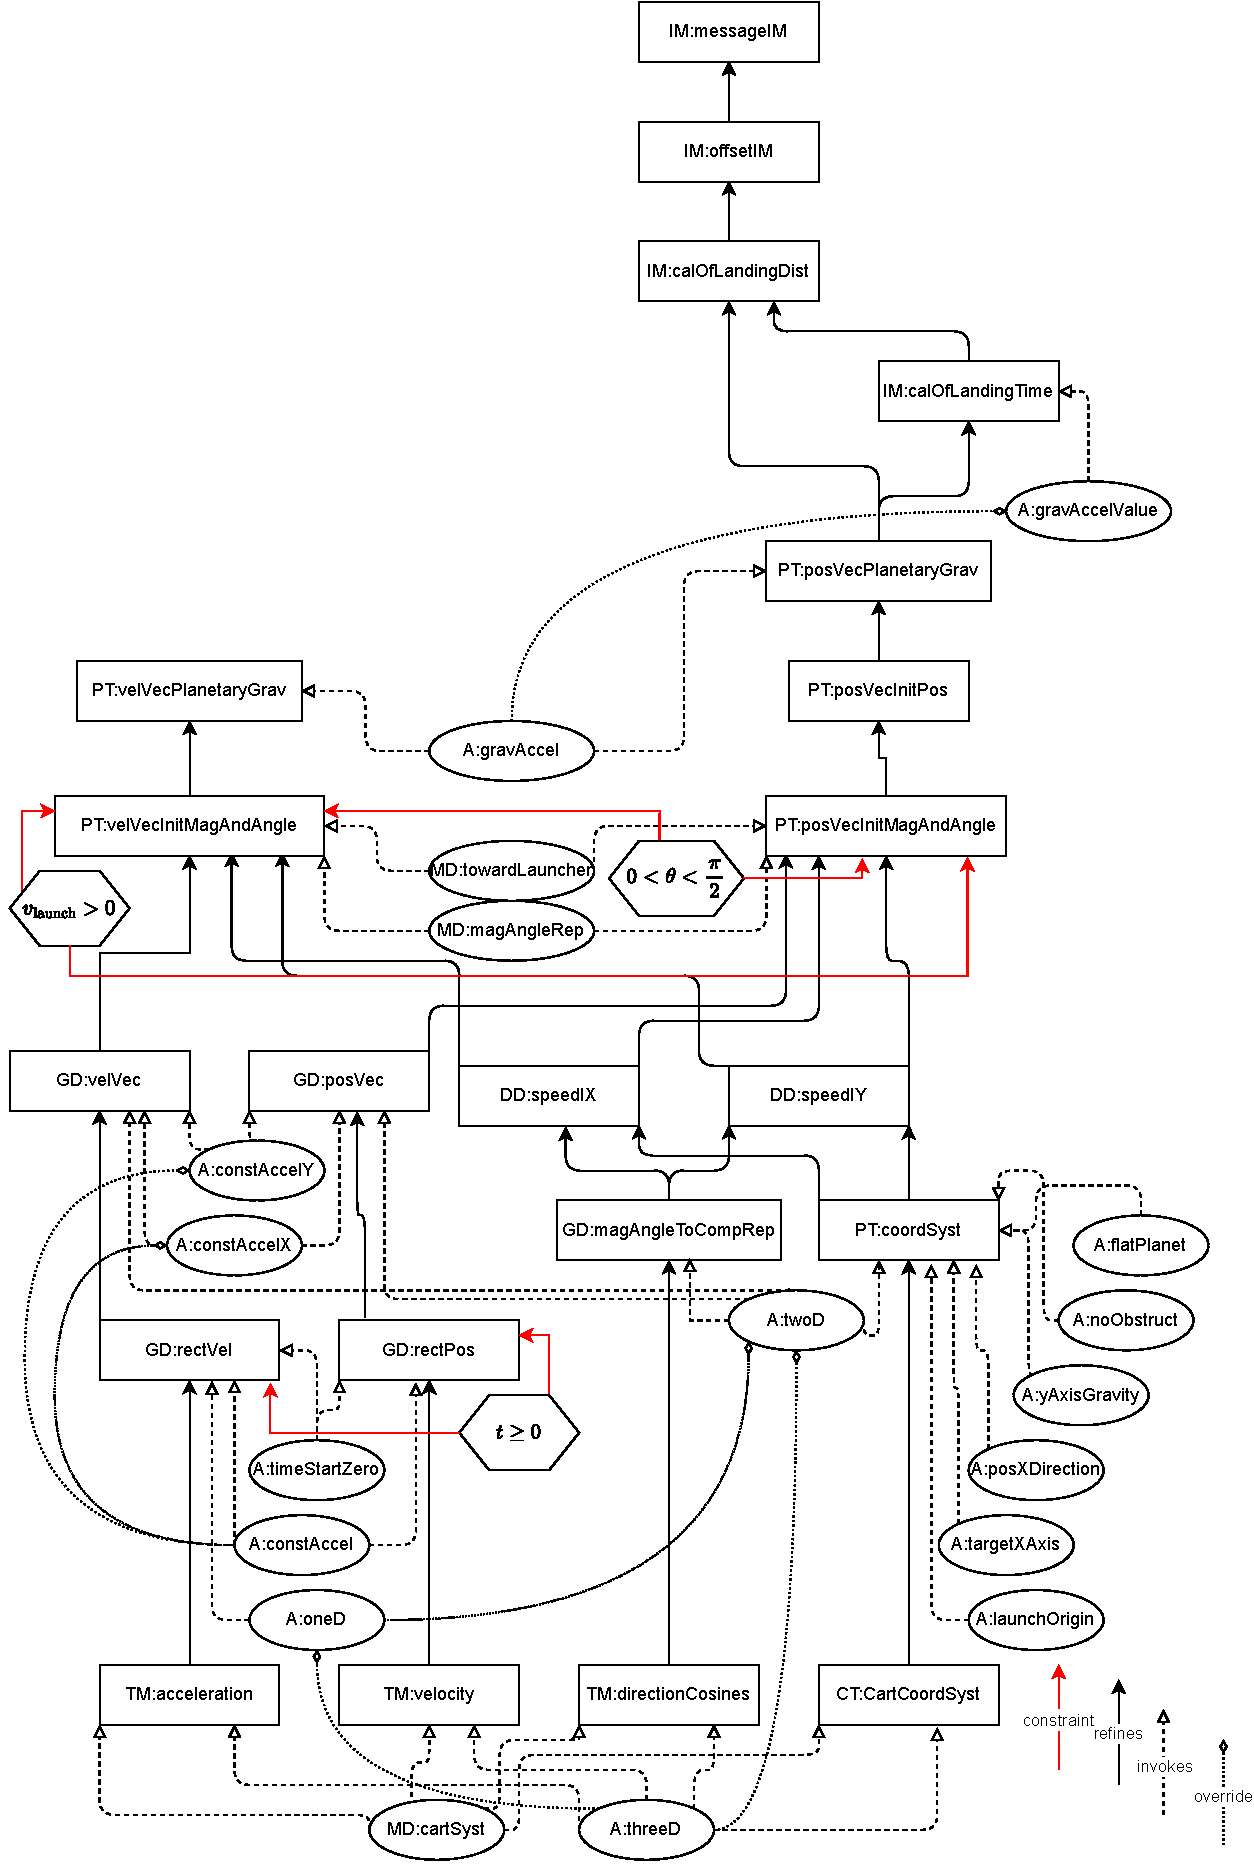
\includegraphics[scale=0.6]{ProjectileTheoriesAssumpts.drawio.pdf}        
\end{center}
\end{figure}

\section{References}
\label{Sec:References}
\begin{filecontents*}{bibfile.bib}
@book{hibbeler2004,
author={Hibbeler, R. C.},
title={Engineering Mechanics: Dynamics},
publisher={Pearson Prentice Hall},
year={2004}}
@mastersthesis{koothoor2013,
author={Koothoor, Nirmitha},
title={A Document Driven Approach to Certifying Scientific Computing Software},
school={McMaster University},
year={2013},
address={Hamilton, ON, Canada}}
@article{parnasClements1986,
author={Parnas, David L. and Clements, P. C.},
title={A rational design process: How and why to fake it},
journal={IEEE Transactions on Software Engineering},
year={1986},
month=feb,
volume={12},
number={2},
pages={251--257},
address={Washington, USA}}
@article{smithKoothoor2016,
author={Smith, W. Spencer and Koothoor, Nirmitha},
title={A Document-Driven Method for Certifying Scientific Computing Software for Use in Nuclear Safety Analysis},
journal={ Nuclear Engineering and Technology},
year={2016},
month=apr,
volume={48},
number={2},
pages={404--418},
howpublished={\url{http://www.sciencedirect.com/science/article/pii/S1738573315002582}}}
@inproceedings{smithLai2005,
author={Smith, W. Spencer and Lai, Lei},
title={A new requirements template for scientific computing},
booktitle={Proceedings of the First International Workshop on Situational Requirements Engineering Processes - Methods, Techniques and Tools to Support Situation-Specific Requirements Engineering Processes, SREP'05},
year={2005},
editor={Agerfalk, PJ and Kraiem, N. and Ralyte, J.},
address={Paris, France},
pages={107--121},
note={In conjunction with 13th IEEE International Requirements Engineering Conference,}}
@article{smithEtAl2007,
author={Smith, W. Spencer and Lai, Lei and Khedri, Ridha},
title={Requirements Analysis for Engineering Computation: A Systematic Approach for Improving Software Reliability},
journal={Reliable Computing, Special Issue on Reliable Engineering Computation},
year={2007},
month=feb,
volume={13},
number={1},
pages={83--107},
howpublished={\url{https://doi.org/10.1007/s11155-006-9020-7}}}
@misc{accelerationWiki,
author={Wikipedia Contributors},
title={Acceleration},
howpublished={\url{https://en.wikipedia.org/wiki/Acceleration}},
month=jun,
year={2019}}
@misc{cartesianWiki,
author={Wikipedia Contributors},
title={Cartesian coordinate system},
howpublished={\url{https://en.wikipedia.org/wiki/Cartesian\_coordinate\_system}},
month=jun,
year={2019}}
@misc{velocityWiki,
author={Wikipedia Contributors},
title={Velocity},
howpublished={\url{https://en.wikipedia.org/wiki/Velocity}},
month=jun,
year={2019}}
\end{filecontents*}
\nocite{*}
\bibstyle{ieeetr}
\printbibliography[heading=none]
\end{document}

TODO

- make assumptions mathematical
- rotation of the Earth assumption
- type for position in 1D, 2D and 3D?
- draw fault tree diagram?
- draw relationship between parts in a graph
- rules - every assumption is invoked and listed, inherited assumptions maintained, or justified or renamed
- table of symbols for final theories?
- data definition - body becomes projectile?